%%%%%%%%%%%%%%%%%%%%%%%%%%%%%%%%%%%%%%%%%%%%%%%%%%%%%%%%%%%%%%%%%%%
%                                                                 %
%   HBOOK User Guide -- LaTeX Source                              %
%                                                                 %
%   Chapter 4                                                     %
%                                                                 %
%   The following external EPS files are referenced:              %
%                                                                 %
%   Editor: Michel Goossens / CN-AS                               %
%   Last Mod.: 10 Sep 1993 20:10 m.g.                             %
%                                                                 %
%%%%%%%%%%%%%%%%%%%%%%%%%%%%%%%%%%%%%%%%%%%%%%%%%%%%%%%%%%%%%%%%%%%
 
\Filename{H1Advanced-features-for-booking-and-editing-operations}
\chapter{Advanced features for booking and editing operations}
\label{HEDITING}
 
\Filename{H2Overview-of-booking-options}
\section{Overview of booking options}

\Subsection{4cm}{\label{HNONEQUI}Histograms with non-equidistant bins}
 
\Shubr{HBOOKB}{(ID,CHTITL,NCX,XBINS,VMX)}
 
\Action As \Rind{HBOOK1}, but instead of giving the lower and upper limits,
        an array \Lit{XBINS} of \Lit{NCX+1} elements is provided.
 
\begin{DLtt}{1234567890123}
\item[XBINS(1)] contains the lower edge of the first bin.
\item[XBINS(2)] contains the lower edge of the second bin.
\item[\quad\ldots] and so on.
\item[XBINS(NCX+1)] contains the upper edge of the last bin.
\end{DLtt}
 
\Subsection{4cm}{\label{HPROFHIS}Profile histograms}
 
\Shubr{HBPROF}{(ID,CHTITL,NCX,XLOW,XUP,YMIN,YMAX,CHOPT)}
\index{profile histogram}
\index{histogram!profile}
 
\Action Create a profile histogram.
Profile histograms are used to display the mean value of Y and
its RMS for each bin in X. Profile histograms are in many cases
an elegant replacement of two-dimensional histograms : the inter-relation
of two measured quantities X and Y can always be visualized
by a two-dimensional histogram or scatter-plot; its representation
on the line-printer is not particularly satisfactory, except
for sparse data. 
If $Y$ is an unknown (but single-valued) approximate
function of $X$, this function is displayed by a profile histogram
with much better precision than by a scatter-plot.
 
The following formulae show the cumulated contents (capital letters)
and the values displayed by the printing or plotting routines
(small letters) of the elements for bin \Lit{J}.
 
\newcommand{\J}{\mathtt{J}}
\[
\begin{array}{r@{\quad=\quad}l@{\qquad\qquad}r@{\quad=\quad}l}
H(\J) &  \sum Y                        &
E(\J) &  \sum {Y^{2}}                  \\
l(\J) &  \sum l                        &
L(\J) &  \sum l                        \\
h(\J) & H(\J)/L(\J)                      &
s(\J) & \sqrt{E(\J)/L(\J)-h(\J)**2}       \\
e(\J) & s(\J)  /  \sqrt {L(\J)}
\end{array}
\]
 
The first five parameters are similar to \Rind{HBOOK1}.
Only the values of Y between \Lit{YMIN} and \Lit{YMAX} will be considered.
To fill a profile histogram,
one must use \Lit{CALL \Rind{HFILL} (ID,X,Y,1.)}.
 
$H(\J)$ is printed as the channel contents.
The errors displayed are $s(\J)$ if \Lit{CHOPT='S'} (spread option),
or $e(\J)$ if \Lit{CHOPT=' '} (error on mean).

\Subsection{4cm}{\label{HROUNDIN}Rounding}

\Shubr{HBINSZ}{('YES'/'NO')}

\Action Round the bin size for bookings of subsequent histograms
to a reasonable value, i.e.:\\
\Lit{1.,1.5,2.,2.5,4.,5.} times an integer power of 10.
\Rind{HBINSZ} controls a switch that, when on, rounds the binsize, still
respecting the number of bins. The switch is
initially off.

\begin{DLtt}{1234567}
\item[{\rm\bf Input parameters:}]
\item['YES'] enable the 'reasonable rounding' feature.
\item['NO'] disable the 'reasonable rounding' feature.
\end{DLtt}

\Subsection{4cm}{\label{HPROSLBA}Projections, Slices, Bands}

\Shubr{HBPRO}{(ID,VMX)}

\Action Books the projections of a 2-dimensional histogram
as two 1-dimensional histograms.

\begin{DLtt}{1234567}
\item[{\rm\bf Input parameters:}]
\item[ID] identifier of an existing 2-dimensional histogram\\
          \Lit{ID=0} means book projections for all existing 2-dimensional
          histograms.
\item[VMX] upper limit of single channel content.
\end{DLtt}
\Remark
\begin{UL}
\item if \Lit{ID} does not exist, or is a 1-dimensional histogram,
      the call does nothing
\item see \Rind{HBOOK1} for details about \Lit{VMX}
\item booking of projections can be executed only after the
      2-dimensional histogram with identifier \Lit{ID} has been booked.
\end{UL}

\Shubrii{HBPROX}{(ID,VMX)}{HBPROY}{(ID,VMX)}
\Action Books projection onto X or Y only.
See \Rind{HBPRO} for more details.
\medskip

\Shubr{HBANDX}{(ID,YMI,YMA,VMX)}

\Action Books a projection onto X, restricted to the Y interval
(\Lit{YMI,YMA}).

\begin{DLtt}{1234567}
\item[{\rm\bf Input parameters:}]
\item[ID] identifier of an existing 2-dimensional histogram
\item[YMI] lower limit of Y interval
\item[YMA] upper limit of Y interval
\item[VMX] maximum value to be stored in 1 channel.
\end{DLtt}
 
The same remarks as for \Rind{HBPRO} apply.
\medskip

\Shubr{HBANDY}{(ID,XMI,XMA,VMX)}

\Action As \Rind{HBANDX} but the projection is onto Y.
\medskip

\Shubr{HBSLIX}{(ID,NSLI,VMX)}

\Action Books slices along Y of 2-dimensional histograms as
\Lit{NSLI} 1-dimensional histograms.\\
Each slice is a projection onto X restricted to an interval
along the Y axis.

\begin{DLtt}{1234567}
\item[{\rm\bf Input parameters:}]
\item[ID]   identifier of an existing 2-dimensional histogram
\item[NSLI] number of slices
\item[VMX]  maximum value to be stored in 1 channel.
\end{DLtt}
 
The same remarks as for \Rind{HBPRO} apply.
\medskip

\Shubr{HBSLIY}{(ID,NSLI,VMX)}

\Action As \Rind{HBSLIX} but slices are projected onto Y.

\Subsection{4cm}{\label{HSTATIS1}Statistics}
Mean value and standard deviation of 1-dimensional histograms
are calculated at editing time, using the channel contents. 
If a more accurate calculation is desired, or if more 
statistical information is needed, the
following option will provide it :
\Lit{CALL HIDOPT (ID,'STAT')}\Iind{STAT}
\medskip

\Shubr{HBARX}{(ID)}

\Action Store the errors for 1-dimensional histograms, X-projections, 
etc., in memory and superimpose them on the plot during output.
This routine must be called after booking {\bf but before filling}.

\begin{DLtt}{12}
\item[{\rm\bf Input parameters:}]
\item[ID] identifier of an existing histogram.
          \Lit{ID=0} means all histograms already booked.
\end{DLtt}

If \Lit{ID} corresponds to a 2-dimensional histogram,
\Rind{HBARX} acts on all X projections, slices, bands.
%  ==========================================================

\NODOC{\begin{minipage}{.49\textwidth}}
\[\mbox{Error}(i) = \sqrt{\sum_{j=1}^{{n^{i}}}\, W_{{ji}}^{2}} \]
\NODOC{\end{minipage} \hfill
\begin{minipage}{.49\textwidth}}
where :\qquad\begin{tabular}[t]{r@{\quad}l}
               $i$        & bin number                     \\
               $n^i$      & number of entries in bin $i$   \\
               $W_{j\,i}$ & weight of event $j$ in bin $i$ \\
              \end{tabular}
\NODOC{\end{minipage}}

It is clear that the sum of the squares of weights in each
bin must also be stored to perform this calculation. However
when filling with weight always equal to 1, errors can be
calculated from bin contents only, and \Rind{HBARX}, \Rind{HBARY}
need not be called. 
The superimposition of error bars can be selected at output time, using
\Lit{HIDOPT(ID,'ERRO')}\Iind{ERRO}
In both cases the values of errors can be printed under the contents,
via the editing option \Lit{HIDOPT(ID,'PERR')}\Iind{PERR}
The entry \Rind{HPAKE} permits user-defined error bar setting.
\medskip

\Shubr{HBARY}{(ID)}
\Action As \Rind{HBARX}, it is used to act on Y
projections of 2-dimensional histograms.
 
\Subsection{4cm}{\label{HFUNCREP}Function Representation}
 
\Shubr{HBFUN1}{(ID,CHTITL,NX,XMI,XMA,FUN)}
 
\Action Books 1-dimensional histogram and fills it with the values of the
external function \Lit{FUN(X)} computed at the centre of each bin.
One computer word per channel is used.
 
The first five parameters are as for \Rind{HBOOK1}.
 
\begin{DLtt}{1234567}
\item[{\rm\bf Input parameters:}]
\item[ID] histogram identifier, integer non zero
\item[CHTITL] histogram title (character variable or constant up to 80
              characters)
\item[NX] number of channels
\item[XMI] lower edge of first channel
\item[XMA] upper edge of last channel
\item[FUN] real function of one variable, to be declared
           \Lit{EXTERNAL} in the calling subroutine, and to be
           supplied by the user.
\end{DLtt}
 
\Shubr{HBFUN2}{(ID,CHTITL,NX,XMI,XMA,NY,YMI,YMA,FUN)}

\Action Books a 2-dimensional
histogram and fills it with the values of the external
function \Lit{FUN(X,Y)}, computed at the centre of each bin.
One computer word per channel is used.
 
The first eight parameters are as for \Rind{HBOOK2}.

\begin{DLtt}{1234567}
\item[{\rm\bf Input parameters:}]
\item[ID] histogram identifier, integer
\item[CHTITL] histogram title  (character variable or constant up to 80
          characters)
\item[NX] number of channels in X
\item[XMI] lower edge of first X channel
\item[XMA] upper edge of last X channel
\item[NY] number of channels in Y
\item[YMI] lower edge of first Y channel
\item[YMA] upper edge of last Y channel
\item[FUN] real function of two variables, to be declared
\Lit{EXTERNAL} in the calling subroutine, and to be supplied by the user.
\end{DLtt}

\Shubr{HFUNC}{(ID,FUN)}

\Action Samples the function \Lit{FUN}, which must have been declared
\Lit{EXTERNAL},
at the centre of the bins of a histogram. The function will be
superimposed onto the histogram at editing time and its values optionally
printed out (see \Lit{HIDOPT(ID,'PFUN')}\Iind{PFUN}
\begin{DLtt}{1234567}
\item[{\rm\bf Input parameters:}]
\item[ID] identifier of an existing 1-dimensional histogram.\\
          \Lit{ID=0} signals that the function should be calculated
          for all existing 1-dimensional histograms.
\item[FUN] External real function, e.g. \Lit{REAL FUNCTION FUN(X)}.\\
          The function parameter \Lit{X}
          will be the central value of a histogram bin. 
          The user must return
          the corresponding function at that point as a value in \Lit{FUN}.
\end{DLtt}

\Remark
\begin{UL}
\item Not existing for 2-dimensional histograms.
\item Function \Lit{FUN}
      cannot contain any call to an entry of the HBOOK package.
\item \Rind{HFUNC}
      can be called several times for the same histogram identifier \Lit{ID}.
      If the latter case, the values of the old function will be
      overwritten by the new one.
\item The chi-squared $\chi^2$, as defined below,
      will be printed along with the statistical
      information at the bottom of the histogram.
\end{UL}
%  ==========================================================
\NODOC{\begin{minipage}{.43\textwidth}}
\[
\chi^{2} = \sum_{i=1}^{n_{ch}}\, 
             \frac{(C(i)-F(i))^2}{\sum_{j=1}^{n^{i}}\, W_{ji}\,^2}
\]
\NODOC{\end{minipage} \hfill
\begin{minipage}{.55\textwidth}}
with:\quad
\begin{tabular}[t]{@{}r@{\quad}l}
$n_{ch}$  & number of channels of histogram                \\
$C(i)$    & contents of channel $i$                        \\
$F(i)$    & value of function at centre of channel $i$     \\
$n^{i}$   & number of entries in channel $i$i              \\
$W_{ji}$  & weight of event $j$ in channel $i$, i.e.       \\
          & square root of contents $C(i)$ or              \\
          & as given by \Rind{HBARX}/\Rind{HPAKE}          \\
\end{tabular}
\NODOC{\end{minipage}}

\newpage%%%%%%%%%%%%%%%%%%%%%%%%%%%%%%%%%%%%%%%%%%%%%%%%%%%%%%%%%%

\subsection{Reserve array in memory}

\Shubr{HARRAY}{(ID,NWORDS,LOC*)}

\Action Reserves an array in the memory storage area managed by HBOOK.

\begin{DLtt}{1234567}
\item[{\rm\bf Input parameters:}]
\item[ID] identifier of the array (pseudo-histogram)
\item[NWORDS] length of the array.
\item[{\rm\bf Output Parameters}]
\item[LOC] Address minus one in the internal \HBOOK{}
           common block \Lit{/PAWC/}
           of the 1st element of the array, i.e.
\index{common {\tt/PAWC/}}\index{PAWC@{\tt/PAWC/} common}
\begin{verbatim}
      COMMON/PAWC/NWPAW,IXPAWC,IHDIV,IXHIGZ,IXKU,FENC(5),LMAIN,HCV(9989)
      DIMENSION IQ(2),Q(2),LQ(8000)
      EQUIVALENCE (LQ(1),LMAIN),(IQ(1),LQ(9)),(Q(1),IQ(1))

      IADDR = Q(LOC+1)
\end{verbatim}
\end{DLtt}

\Remark
At any time the address of preudo-histogram \Lit{ID} can
be obtained with \Lit{\Rind{HLOCAT}(ID,LOC)}

\newpage%%%%%%%%%%%%%%%%%%%%%%%%%%%%%%%%%%%%%%%%%%%%%%%%%%%%%%%%%%

\subsection{Axis labels and histograms}

A set of routines, \Rind{HLABEL}, \Rind{HFC1} and \Rind{HFC2},
allows one to associate labels with histogram channels.
This association can be made before or after a histogram is filled, but 
it has the advantage that the label information get stored in the
histogram data structure, so that it is available for all future plots in
an automatic way in the HPLOT and PAW packages.
\index{PAW}\index{HPLOT}
Printing histograms with associated alphanumeric
labels is not implemented in the
line-printer oriented routines of HBOOK.

\Shubr{HLABEL}{(ID,NLAB,*CLAB*,CHOPT)}

\Action 
Associates alphanumeric labels with a histogram.
This routine can be called for a histogram after it has been filled,
and then the labels specified will be shown on the respective axes.
The routine can also be called before a histogram is filled ,
and in this case, when filling, a certain order can be imposed.
By default the entries will be automatically ordered.

\begin{DLtt}{123456}
\item[{\rm\bf Input parameters:}]
\item[ID]     Histogram identifier.
\item[NLAB]   Number of labels.
\item[CHOPT]  Character variable specifying the option desired.
              \begin{DLtt}{123}
                \item[' '] As \Lit{'N'} below.
                \item['N'] Add \Lit{NLAB} new labels read in \Lit{CLAB}
                           to histogram \Lit{ID}.
                \item['R'] Read \Lit{NLAB} labels into in \Lit{CLAB}
                           from histogram \Lit{ID}.
                \item['X'] X-axis is being treated (default).
                \item['Y'] Y-axis is being treated.
                \item['Z'] Z-axis is being treated.
                \item['S'] Sorting order of the labels:
                           \begin{DLtt}{123}
                             \item['S']  default, as \Ropt{SA};
                             \item['SA'] alphabetically;
                             \item['SE'] reverse alphabetical order;
                             \item['SD'] by increasing channel contents
                                         (after filling);
                             \item['SV'] by decreasing channel contents
                                         (after filling).
                           \end{DLtt}
                \item['T'] Modify (replace) \Lit{NLAB} existing labels read from 
                           \Lit{CLAB} in histogram \Lit{ID}.
              \end{DLtt}
\item[{\rm\bf Input/Output parameter:}]
\item[*CLAB*] Character variable array with
              \Lit{NLAB} elements (input and output).
\end{DLtt}

Notes:
\begin{UL}
\item For one-dimensional histograms \Rind{HLABEL} can be called at any time.
\item For two-dimensional histograms one {\bf must} call \Rind{HLABEL}
      with option \Lit{'N'} for each axis between the call to \Rind{HBOOK2}
      and the first call to \Rind{HFC2}.
\end{UL}

\newpage%%%%%%%%%%%%%%%%%%%%%%%%%%%%%%%%%%%%%%%%%%%%%%%%%%

\Filename{H2Filling-Operations}
\Section{4cm}{Filling Operations}
\label{HOTHFILL}

It is possible to speed up the filling process with the loss 
of some protection,
and to globally transfer an array or a matrix to a histogram.

\Subsection{4cm}{Fast Filling Entries}
\label{HFASTFIL}
 
If the program that is using HBOOK fills many histograms several
times a substantial fraction of time can be spent by \Rind{HFILL}
in searching for the histogram it has to fill, deciding which type
of histogram
it is and unpacking and packing bits if more than one channel is to
be stored in one computer word.
To reduce the overall filling time, there are several actions
that can be taken
 
\begin{UL}
\item Bypass part of the logic that finds out the characteristics
of the histogram to fill. This can be achieved by using,
instead of \Rind{HFILL}
the special filling entries described in this section.
\item Avoid packing more than one channel in a computer word.
\end{UL}
 
For these reasons it is recommended to use always \Rind{HFILL}
at the development stage, and replace it later with
\Rind{HF1}, \Rind{HF2}, etc. only when a rather 
stable program is going to be used extensively.
 
Calls to \Rind{HFILL} and \Rind{HF1} or \Rind{HF2}
cannot be mixed on the same \Lit{ID}.
\medskip
 
\Shubr{HF1}{(ID,X,WEIGHT)}
 
\Action Analogous to \Rind{HFILL} on a 1-dimensional histogram
but \Rind{HBARX} and \Lit{HIDOPT(ID,'STAT')}\Iind{STAT} are ignored.
 
\begin{DLtt}{1234567}
\item[{\rm\bf Input parameters:}]
\item[ID] histogram identifier
\item[X] value of the abscissa
\item[WEIGHT] event weight
\end{DLtt}
 
\Shubr{HF1E}{(ID,X,WEIGHT,ERRORS)}
 
\Action Analogous to \Rind{HF1}, but also the errors are accumulated.
 
\begin{DLtt}{1234567}
\item[{\rm\bf Input parameters:}]
\item[ID] histogram identifier.
\item[X] value of the abscissa.
\item[WEIGHT] the content is incremented by \Lit{WEIGHT}.
\item[ERROR] the error is incremented by \Lit{ERROR**2}.
\end{DLtt}
 

===>  HF1E Fills a 1-D histogram

      SUBROUTINE HF1E(ID,X,W,E)

      - ID : Histogram identifier.
      - X  : Value of the abscissa
      - W  : Content is incremented by W
      - E  : Errors is incremented by E**2


\Shubr{HF2}{(ID,X,Y,WEIGHT)}
 
\Action 
Analogous to \Rind{HFILL}
on a 2-dimensional histogram except that projections,
bands, slices are not filled. 
\Rind{HBARY} is ignored as well.
 
\begin{DLtt}{1234567}
\item[{\rm\bf Input parameters:}]
\item[ID] histogram identifier
\item[X] value of the abscissa
\item[Y] value of the ordinate
\item[WEIGHT] event weight
\end{DLtt}
 
\Shubr{HFF1}{(ID,*NID*,X,WEIGHT)}
 
\Action 
Analogous to \Rind{HF1} with the same restrictions.
 
\begin{DLtt}{1234567}
\item[{\rm\bf Input parameters:}]
\item[ID]     histogram identifier
\item[NID]    is a histogram-specific variable that has to
              be provided by the user.\\
              Before the first call, \Lit{NID} must be initialized to 0.\\
              In subsequent calls to \Rind{HFF1} the constant
              \Lit{NID} must then be used in order
              to skip the calculation of the histogram address.
\item[X]      value of the abscissa
\item[WEIGHT] event weight
\item[{\rm\bf Output parameter:}]
\item[NID]    After the first call to \Rind{HFF1},
              \Lit{NID} will contain the current address
              of histogram \Lit{ID}.
\end{DLtt}
 
\Shubr{HFF2}{(ID,NID,X,Y,W)}
 
\Action Analogous to \Rind{HF2} with the use of the parameter
\Lit{NID} as explained for \Rind{HFF1}
 
\Shubr{HFPAK1}{(ID,NID,V,N)}
 
\index{histogram!packing}
\index{packing}
\index{floating number}
 
\Action Fill an histogram using the contents of a vector.
 
\begin{DLtt}{1234567}
\item[{\rm\bf Input parameters:}]
\item[ID] histogram identifier
\item[V] array containing the values to be entered into the histogram.
\item[N] length (dimension) of the array \Lit{V}
\item[{\rm\bf Input/output parameter:}]
\item[*NID*] address of histogram (see \Rind{HFF1})
\end{DLtt}
 
This subroutine has the same effect as
 
\begin{verbatim}
   DO 10 I=1,N
10 CALL HFF1(ID,NID,V(I),1.)
\end{verbatim}
 
where the array \Lit{V} of \Lit{N} words must have been filled
previously by the user.
\medskip
 
\Shubr{HIPAK1}{(ID,NID,IV,N)}
 
\index{histogram!packing}
\index{packing}
\index{integer number}
 
\Action 
Analogous to \Rind{HFPAK1}, except that the user vector contains now
integers instead of real numbers.
 
\Subsection{4cm}{\label{HGLOBFIL}Global Filling}
 
A vector or matrix can be transferred into a histogram with a single call.
 
\Shubr{HPAK}{(ID,CONTEN)}
 
\index{histogram!packing}
\index{packing}
\index{array}
 
\Action 
Transfer the contents of an array as channel contents into an
histogram. The original contents of the histogram are overwritten.
 
\begin{DLtt}{1234567}
\item[{\rm\bf Input parameters:}]
\item[ID] an existing histogram identifier
\item[CONTEN] a user array, suitably dimensioned
\end{DLtt}
 
\Remark
 
\begin{UL}
\item In the case of a {\bf 1-dimensional} histogram, the dimension
      of the array must at least be equal to the number of
      histogram channels (\Lit{NCHAN}), i.e.
      \Lit{DIMENSION CONTEN(NX)} with \Lit{NX}$>$\Lit{NCHAN}
\item In the case of a {\bf 2-dimensional} histogram, the dimensions
      of the array must exactly be equal to the number of
      histogram channels (\Lit{NCHANX} and \Lit{NCHANY}), \\
      i.e. \Lit{DIMENSION CONTEN(NX,NY)} with \Lit{NX=NCHAN} and 
      \Lit{NY=NCHANY}\\
      Projections and slices, if present for the given histogram,
      are {\bf not} filled.
\index{projection}
\index{slice}
\end{UL}
 
\Shubr{HPAKAD}{(ID,CONTEN)}
 
\index{histogram!packing}
\index{packing}
\index{array}
 
\Action 
Similar to \Rind{HPAK}, but instead of overwriting the
channel contents, the array values are {\bf added} to the
respective channel contents.
 
\Shubr{HPAKE}{(ID,ERRORS)}
 
\index{histogram!packing}
\index{packing}
\index{error}
 
\Action 
Store the contents of an array 
as the errors for the bins of the 1-dimensional histogram for
which the option \Rind{HBARX} has been invoked.
 
\begin{DLtt}{1234567}
\item[{\rm\bf Input parameters:}]
\item[ID] histogram identifier
\item[ERRORS] user array containing the errors to be assigned to the
       histogram bin contents. Its dimension should be at least equal to
       the number of channels in histogram \Lit{ID}.
\end{DLtt}
 
\Remark
 
If the \Rind{HBARX} option was not set for the given histogram, then
it is activited by a call to \Rind{HPAKE}.

\newpage%%%%%%%%%%%%%%%%%%%%%%%%%%%%%%%%%%%%%%%%%%%%%%%%%%%%%%

\subsection{Filling histograms using character variables}

Routines for which, using routine \Rind{HLABEL}, alphanumeric 
labels were associated with the histogram channels, 
are filled with the routines \Rind{HFC1} and \Rind{HFC2}.
These allow, on top of by bin number, 
to fill an histogram by specifying a alphanumeric channel identifier.

\Shubr{HFC1}{(ID,IBIN,CLAB,W,CHOPT)}

\Action Fills a channel in a one-dimensional histogram.

\begin{DLtt}{12345}
\item[ID]     One-dimensional histogram identifier.
\item[IBIN]   Number of the bin to be filled (if $\ne0$).
\item[CLAB]   Character variable containing the label 
              describing the bin (if \Lit{IBIN=0}).
\item[CHOPT]  Character variable specifying the option desired.
              \begin{DLtt}{12}
                \item[' '] default, as \Ropt{S};
                \item['N'] filling order, i.e. the order of the labels on the
                           plot is given by the sequence in which they are
                           presented in the successive calls to the routine
                           (this method can be very time consuming since all
                           channels must be scanned at each call);
                \item['S'] automatic sort;
                \item['U'] if the channel does not exist 
                           then the underflow channel is incremented
                           (by default a new channel is created for each new label).
                \end{DLtt}
\end{DLtt}

\Remarks
\begin{UL}
\item If \Lit{IBIN\(\ne\)0}, then the channel \Lit{IBIN}
      is filled; \Lit{CLAB} may then be undefined.
\item When a label is encountered, which is not yet known, then for options \Lit{'N'} 
      and \Lit{'S'} a new channel is added dynamically, while for option 
      \Ropt{U} the underflow channel is incremented.
\item Routine \Rind{HLABEL} can be called  before or after \Lit{HFC1}.
\end{UL}

\Shubr{HFC2}{(ID,IBINX,CLABX,IBINY,CLABY,W,CHOPT)}

\Action Fills for a two-dimensional histogram the channel identified
by position \Rarg{IBINX} or label \Rarg{CLABX} and
position \Rarg{IBINY} or label \Rarg{CLABY} with weight \Rarg{W}.

\begin{DLtt}{12345}
\item[ID]     Two-dimensional histogram identifier.
\item[IBINX]  Number of the X-bin to be filled (if $\ne0$).
\item[CLABX]  Character variable containing the label 
              describing the X-bin (if \Rarg{IBINX=0}).
\item[IBINY]  Number of the Y-bin to be filled (if $\ne0$).
\item[CLABY]  Character variable containing the label 
              describing the Y-bin (if \Rarg{IBINY=0}).
\item[W]      Weight of the event to be entered into the histogram.
\item[CHOPT]  Character variable specifying the option desired.
              \begin{DLtt}{123}
                \item[' '] default, as \Ropt{S};
                \item['N'] filling order (see \Rind{HFC1};
                \item[S]   automatic sort (default)
                \item['U'] if the channel does not exist 
                           then the underflow channel is incremented
                           (by default a new channel is created for each new label).
                \end{DLtt}
\end{DLtt}

\newpage%%%%%%%%%%%%%%%%%%%%%%%%%%%%%%%%%%%%%%%%%%%%%%%%%%

\Remarks
\begin{UL}
\item For efficiency reasons, routine \Rind{HLABEL} must be called  
      {\bf before} \Rind{HFC2}.
\item If \Lit{IBINX\(\ne\)0}, then the channel described by \Rarg{IBINX}
      is filled; \Lit{CLABX} may then be undefined.  
\item If \Lit{IBINY\(\ne\)0}, then the channel described by \Lit{IBINY}
      is filled; \Lit{CLABY} may then be undefined.  
\item If the channel described by \Lit{IBINX} or \Lit{CLABX} does not exist,
      the underflow channel is incremented. Idem for \Lit{IBINY} and \Lit{CLABY}.
\end{UL} 

The example below shows different uses of the label routines.
The input data are the same as those used for building the Ntuple
on page~\pageref{sec:ntuplestaff}.
Three histograms are booked. For the first one (\Lit{11}), the number
of channels (\Lit{13}) is given explicitly, and a call to \Rind{HLABEL}
declares all the labels for that histogram.
Then a second histogram (\Lit{12}) is booked with one pre-declared channel.
In fact this latter histogram will be filled with \Rind{HFC1}, in a way
completely identical to histogram \Lit{11}, 
but channels will be dynamically added as new labels are encountered.
We also create a 2-D histogram (\Lit{21}), where for the y-axis we
again pre-declare labels and we fill it with a call to \Rind{HFC2}.
After the loop, where the histograms are filled, we tell HBOOK to
order the labels in the second histogram (\Lit{12}) according to
decreasing bin contents.
This shows that it is not necessary, in the 1-D case, to
pre-declare the labels of a histogram, but that they can be
added to a histogram ``on the fly'', i.e. while filling.
The sorting order can be specified after the histogram is filled.
As stated earlier, labels are only printed on graphical output devices,
so that one must use HPLOT/HIGZ to see the effect of the label routines.
The calls to the HPLOT/HIGZ routines, used to generate the PostScript
picture shown in Fig.~\ref{fig:HLABEL}, are described in the HIGZ/HPLOT
manual.

\newpage

\begin{XMPt}{Example of the use of the histogram label routines}
\NODOC{\baselineskip.95\baselineskip\relax}      PROGRAM CERN

      PARAMETER (NWPAWC = 30000)
      COMMON /PAWC/ IPAW(NWPAWC)
      REAL        RDATA(11)
      CHARACTER*4 CHDIV,CHDIVS(13), CHNAT,CHNATS(15)

      DATA CHDIVS /'AG', 'DD', 'DG', 'EF', 'EP', 'FI', 'LEP', 'PE',
     +           'PS', 'SPS', 'ST', 'TH', 'TIS'/
      DATA CHNATS /'AT', 'BE', 'CH', 'DE', 'DK', 'ES', 'FR', 'GB',
     +           'GR', 'IT', 'NL', 'NO', 'PT', 'SE', 'ZZ'/

      CALL HLIMIT(NWPAWC)
*
      OPEN(11,FILE='aptuple.dat', STATUS='OLD')
      OPEN(12,file='hlabexa.ps',form='formatted',status='unknown')

      CALL HBOOK1(11,'Example HLABEL explicit list',13,1.,14.,0.)
      CALL HBOOK1(12,'Example HLABEL implicit list',1 ,0.,1. ,0.)
      CALL HBOOK2(21,'Example HLABEL 2-D',13,2.,15.,13,1.,14.,0.)
*
      CALL HLABEL(11,13,CHDIVS,'N')
      CALL HLABEL(21,13,CHDIVS,'NY')
*
*-- Loop over input data
*
      DO 10 IEVENT = 1, 99999
         READ(11, '(10F4.0, F7.0)', END=20) RDATA
         CHDIV    = CHDIVS(INT(RDATA(2)))
         IGRADE   = RDATA(7)
         CALL HFC1(11,0,CHDIV,1.,' ')
         CALL HFC1(12,0,CHDIV,1.,' ')
         CALL HFC2(21,IGRADE,' ',0,CHDIV,1.,' ')
   10 CONTINUE
      
   20 CALL HLABEL(12,0,' ','SV')  
*
*-- Call the HPLOT/HIGZ routines to print the histos showing the labels
*
      CALL HPLINT(0)
      CALL HPLCAP(-12)
      CALL HPLSET('VSIZ',0.20)
      CALL HPLSET('NDVX',-13.05)
      CALL HPLSET('HCOL',1105)
      CALL HPLSET('BCOL',1.5)
      CALL HPLSET('*FON',-60.)
      CALL HPLOPT('NBOX',1)
      CALL HPLZON(2,2,1,' ')
      CALL HPLOT(11,' ',' ',0)
      CALL HPLOT(12,' ',' ',0)
      CALL HPLZON(1,2,2,'S')  
      CALL HPLOPT('GRID',1)
      CALL HPLOT(21,'BOX',' ',0)
      CALL HPLEND
*
      END
\end{XMPt}

%\subsubsection*{Operations on histogram labels}
%
%\begin{XMP}
%\begin{Bcommand}
%LOGICAL FUNCTION HLABEQ (ID,CHOPT)
%\end{Bcommand}
%\end{XMP}
%
%Varifies whether a histogram has labels.
%
%\begin{DLtt}{12345}
%\item[ID]     Histogram identifier.
%\item[CHOPT]  Character variable specifying the option desired.
%              \begin{DLtt}{123}
%                \item[' '] return \Lit{.true.} if histogram \Lit{ID}
%                    has labels, else return \Lit{.false.};
%               \item['X'] return \Lit{.true.} if X axis
%                    has labels, else return \Lit{.false.};
%               \item['Y'] return \Lit{.true.} if Y axis
%                    has labels, else return \Lit{.false.};
%              \end{DLtt}
%\end{DLtt}
%
%\begin{XMP}
%\begin{Bcommand}
%INTEGER FUNCTION HLABNB (ID,CHOPT)
%\end{Bcommand}
%\end{XMP}
%
%Returns the number of labels for the axes of
%a histogram.
%
%\begin{DLtt}{12345}
%\item[ID]     Histogram identifier.
%\item[CHOPT]  Character variable specifying the option desired.
%              \begin{DLtt}{123}
%                \item[' '] like \Lit{'X'} below;
%               \item['X'] return the number of labels for the X axis;
%               \item['Y'] return the number of labels for the Y axis;
%              \end{DLtt}
%\end{DLtt}
%
%\begin{XMP}
%\begin{Bcommand}
%CALL HLGNXT (ID,IBIN,CLAB*,CHOPT)
%\end{Bcommand}
%\end{XMP}
%
%Get channel label from channel number.
%
%\begin{DLtt}{12345}
%\item[ID]     Histogram identifier.
%\item[IBIN]   Number of the channel.
%\item[CLAB*]  Character variable (CHARACTER*16) containing the label 
%              corresponding to channel \Lit{IBIN} (output variable).
%\item[CHOPT]  Character variable specifying the axis desired.
%              \begin{DLtt}{123}
%               \item[' '] As \Lit{'X'} below;
%               \item['X'] Get label of X axis;
%               \item['Y'] Get label of Y axis;
%               \item['Z'] Get label of Z axis.
%              \end{DLtt}
%\end{DLtt}
%
%\begin{XMP}
%\begin{Bcommand}
%CALL HLPOS (ID,CHLAB,IBIN*,CLAB,CHOPT)
%\end{Bcommand}
%\end{XMP}
%
%Get channel number from channel label.
%
%\begin{DLtt}{12345}
%\item[ID]     Histogram identifier.
%\item[CLAB]   Character variable (CHARACTER*16) specifying the label 
%              one is looking for.
%\item[IBIN*]  Number of the channel (output variable).
%              If no channel has label \Lit{CLAB} a value \Lit{IBIN=-1}
%              is returned.
%\item[CHOPT]  Character variable specifying the axis desired.
%              \begin{DLtt}{123}
%               \item[' '] As \Lit{'X'} below;
%               \item['X'] Get label of X axis;
%               \item['Y'] Get label of Y axis;
%               \item['Z'] Get label of Z axis.
%              \end{DLtt}
%\end{DLtt}
%
%*     Changes in HSCR to delete ntuples
%      SUBROUTINE HSCR(IDD,ICYCLE,CHOPT)
%*.==========>
%*.           To scratch histogram ID from current directory
%*.           /PAWC/ or RZ file. IDD =0 means all histograms.
%*.           ICYCLE is the cycle number in case of a RZ file.
%*..=========>
%*
%*     New routine HDDIR to delete directories (memory or RZ)
%      SUBROUTINE HDDIR(CHDIR)
%*.==========>
%*.            Delete sub-directory CHDIR from /PAWC/  or RZ file.
%*.            The current directory must be the mother directory of CHDIR
%*..=========>
%*
%
%
\begin{figure}[btp]
\epsfig{file=hlabel.eps,width=\textwidth}
\caption{Example of the use of \protect\Rind{HLABEL}}
\label{fig:HLABEL}

\begin{UL}
\item The top left picture shows the contents of the histogram ordered
      alphabetically by label.
\item The top right picture shows the same histogram, but with the 
      bins ordered by decreasing contents, irrespective of their label.
\item The lower picture shows a two-dimensional histogram,
      where the ordinate (Y-axis) ordered alphabetically.
\end{UL}
\end{figure}


\clearpage%%%%%%%%%%%%%%%%%%%%%%%%%%%%%%%%%%%%%%%%%%%%%%%%%%%%%%%

\begin{XMPt}{Example of booking options}
      SUBROUTINE HEXAM2
*.==========>
*.           TEST OF SOME BOOKING OPTIONS USING HBOOK RANDOM
*.           NUMBER GENERATORS.
*..=========> ( R.Brun )
      COMMON/HDEXF/C1,C2,XM1,XM2,XS1,XS2
      DOUBLE PRECISION C1,C2,XM1,XM2,XS1,XS2
      EXTERNAL HTFUN1,HTFUN2
*.___________________________________________
*.
*             Booking
*
      C1=1.
      C2=0.5
      XM1=0.3
      XM2=0.7
      XS1=0.07
      XS2=0.12
*
      CALL HBFUN1(100,'TEST OF HRNDM1',100,0.,1.,HTFUN1)
      CALL HIDOPT(100,'STAR')
      CALL HCOPY(100,10,' ')
*
      CALL HBOOK1(110,  'THIS HISTOGRAM IS FILLED ACCORDING TO THE FUNCT
     +ION HTFUN1'
     +  ,100,0.,1.,1000.)
*
      CALL HBFUN2(200,'TEST OF HRNDM2',100,0.,1.,40,0.,1.,HTFUN2)
      CALL HSCALE(200,0.)
      CALL HCOPY(200,20,' ')
*
      CALL HBOOK2(210,'HIST FILLED WITH HFILL AND HRNDM2' ,100,0.,1.,
     +  40,0.,1.,30.)
*
*             Filling
*
      DO 10 I=1,5000
         X=HRNDM1(100)
         CALL HFILL(110,X,0.,1.)
         CALL HRNDM2(200,X,Y)
         CALL HFILL(210,X,Y,1.)
  10  CONTINUE
*
*             Save all histograms on file 'hexam.dat'
*
      CALL HRPUT(0,'hexam.dat','N')
*
      CALL HDELET(100)
      CALL HDELET(200)
*
*             Printing
*
      CALL HPRINT(0)
      END
      FUNCTION HTFUN1(X)
      DOUBLE PRECISION HDFUN1
      HTFUN1=HDFUN1(X)
      END
      FUNCTION HTFUN2(X,Y)
      HTFUN2=HTFUN1(X)*HTFUN1(Y)
      END
      DOUBLE PRECISION FUNCTION HDFUN1(X)
      COMMON/HDEXF/C1,C2,XM1,XM2,XS1,XS2
      DOUBLE PRECISION C1,C2,XM1,XM2,XS1,XS2,A1,A2,X1,X2
*
      A1=-0.5*((X-XM1)/XS1)**2
      A2=-0.5*((X-XM2)/XS2)**2
      IF(A1.LT.-20.)THEN
         X1=0.
      ELSEIF(A1.GT.20.)THEN
         X1=1.E5
      ELSE
         X1=C1*EXP(A1)
      ENDIF
      IF(A2.LT.-20.)THEN
         X2=0.
      ELSEIF(A2.GT.20.)THEN
         X2=1.E5
      ELSE
         X2=C2*EXP(A2)
      ENDIF
      HDFUN1=X1+X2
      END
\end{XMPt}
\newpage
\begin{Listing}
 TEST OF HRNDM1                                                                  
 
 HBOOK     ID =        10                                        DATE  17/12/91              NO =   4
 
       10                                   ****
        9.75
        9.5                                *    *
        9.25
        9                                 *      *
        8.75
        8.5
        8.25                             *        *
        8
        7.75
        7.5                             *          *
        7.25
        7
        6.75                           *            *
        6.5
        6.25
        6                                            *
        5.75                          *
        5.5
        5.25
        5                            *                *                           ********
        4.75                                                                    **        **
        4.5                                                                    *            *
        4.25                                           *                      *              *
        4                           *                                        *                *
        3.75                                                                *                  *
        3.5                                             *                  *                    *
        3.25                       *                                      *                      *
        3                                                *               *                        *
        2.75                      *                                     *                          *
        2.5                                               *            *                            *
        2.25                     *                                    *                              *
        2                                                  *        **                                *
        1.75                    *                           *      *                                   **
        1.5                                                  ******                                      *
        1.25                   *                                                                          **
        1                     *                                                                             *
         .75                 *                                                                               ***
         .5                **                                                                                   ***
         .25    ***********                                                                                        *
 
 CHANNELS 100   0                                                                                                  1   
           10   0        1         2         3         4         5         6         7         8         9         0   
            1   1234567890123456789012345678901234567890123456789012345678901234567890123456789012345678901234567890   
 
 CONTENTS   1.                 11223345678899999988765443221111111111122223333444444444444444433332222111111        
 *10**  1   0   0000000001234681505297653183799848145791483964333346791469146813567899998765318641964197531087654322
            0   0000123583003267539488304339899027929647999998500671879261615911069969969960119505050742236063223694
            0   1247315797649110704725408821516203649039012333618823383230115137101215512101720499659126352424226173
            0   4557197143534774472257850306737109143583172717457650550628417019558717717855896970455185631419095996
 
 LOW-EDGE   1.            111111111122222222223333333333444444444455555555556666666666777777777788888888889999999999
 *10**  1   0   0123456789012345678901234567890123456789012345678901234567890123456789012345678901234567890123456789
 
 * ENTRIES =        100      * ALL CHANNELS = 0.3249E+02      * UNDERFLOW = 0.0000E+00      * OVERFLOW = 0.0000E+00
 * BIN WID = 0.1000E-01      * MEAN VALUE   = 0.4830E+00      * R . M . S = 0.2198E+00
 
\newpage
 THIS HISTOGRAM IS FILLED ACCORDING TO THE FUNCTION HTFUN1                       
 
 HBOOK     ID =       110                                        DATE  17/12/91              NO =   5
 
      172                                    -
      168                                    I
      164                                    I
      160                                   -I
      156                                   II -
      152                                   II-I
      148                                   I  I-
      144                                 --I   I
      140                                 I     I-
      136                                 I      I
      132                                 I      I
      128                                 I      I-
      124                                -I       I
      120                               -I        I
      116                               I         I
      112                               I         I
      108                               I         I
      104                              -I         I-
      100                              I           I
       96                              I           I -
       92                              I           I-I
       88                             -I             I
       84                             I              I -                              - -
       80                             I              I I                        -     I I  -
       76                             I              I I                        I--  -I I  I
       72                             I              I I-                       I I- II I  I -
       68                             I              I-II                    -  I  I-II-I--I-I
       64                             I                 I                  --I  I            I-
       60                           - I                 I                  I I -I             I
       56                           I-I                 I                  I I-I              I -
       52                           I                   I-               --I                  I-I
       48                          -I                    I-              I                      I
       44                          I                      I             -I                      I-  -
       40                          I                      I-           -I                        I  I
       36                          I                       I           I                         I--I-
       32                          I                       I    -     -I                             I
       28                         -I                       I- - I -  -I                              I- -
       24                       --I                         I-I I I- I                                I I--
       20                      -I                             I I-II-I                                I-I I -
       16                      I                              I-I                                         I-I
       12                     -I                                                                            I--
        8                 - --I                                                                               I----
        4            -----I-I                                                                                     I-
 
 CHANNELS 100   0                                                                                                  1   
           10   0        1         2         3         4         5         6         7         8         9         0   
            1   1234567890123456789012345678901234567890123456789012345678901234567890123456789012345678901234567890   
 
 CONTENTS 100                          1111111111111                                                                
           10                 112224658012445755432099687543222121221233455666557776678686676664543343222221111     
            1.       21124626818147606828212710478511552225771649871850922032539736953183588893942434650812591167574
 
 LOW-EDGE   1.            111111111122222222223333333333444444444455555555556666666666777777777788888888889999999999
 *10**  1   0   0123456789012345678901234567890123456789012345678901234567890123456789012345678901234567890123456789
 
 * ENTRIES =       5000      * ALL CHANNELS = 0.5000E+04      * UNDERFLOW = 0.0000E+00      * OVERFLOW = 0.0000E+00
 * BIN WID = 0.1000E-01      * MEAN VALUE   = 0.4834E+00      * R . M . S = 0.2184E+00
\newpage
 TEST OF HRNDM2                                                                  
 
 HBOOK     ID =        20                                        DATE  17/12/91              NO =   6
 
 CHANNELS 100 U 0                                                                                                  1 O 
           10 N 0        1         2         3         4         5         6         7         8         9         0 V 
            1 D 1234567890123456789012345678901234567890123456789012345678901234567890123456789012345678901234567890 E 
            ************************************************************************************************************
   OVE      *                                                                                                          * OVE
      .975  *             ..........................................................................................   *  40
      .95   *           ..................++++++++..................................................................   *  39
      .925  *          ................+++++++++++++++..............................................................   *  38
      .9    *          .............+++++2222222222+++++.....................++++++++++++++++++.....................   *  37
      .875  *         .............+++2223333333333222++++...............++++++++++++++++++++++++++.................   *  36
      .85   *        ............++++2233444444444433222+++...........++++++++2222222222222222++++++++..............   *  35
      .825  *        ...........+++2233445566666655443322++++......+++++++222222233333333332222222++++++............   *  34
      .8    *       ............++223345567778877765543322++++++++++++++2222233333333443333333322222++++++..........   *  33
      .775  *       ...........+++2334567788999998776544322+++++++++++22223333344444444444444333332222+++++.........   *  32
      .75   *       ...........++2234567889AAAAAA98876543322+++++++++2222333344445555555555444433332222+++++........   *  31
      .725  *       ..........+++233456789ABBBBBBA98765443222+++++++222233344445555555555555544443332222+++++.......   *  30
      .7    *       ..........+++23445789AABCCCCBBA9876543222++++++2222333344455555666666555554443332222+++++.......   *  29
      .675  *       ..........+++23445789AABCCCCBBA9876543222++++++2222333344455555666666555554443332222+++++.......   *  28
      .65   *       ..........+++233456789ABBBBBBA98765443222+++++++222233344445555555555555544443332222+++++.......   *  27
      .625  *       ...........++2234567889AAAAAA98876543322+++++++++2222333344445555555555444433332222+++++........   *  26
      .6    *       ...........+++2334567789999998776544322+++++++++++22223333344444444444444333332222+++++.........   *  25
      .575  *       ............++223345567778877765543322++++++++++++++2222233333333443333333322222++++++..........   *  24
      .55   *        ...........+++2233445566666655443322++++......+++++++222222233333333332222222++++++............   *  23
      .525  *        ............+++22233444455444433222++++.........+++++++++2222222222222222++++++++..............   *  22
      .5    *         ............++++2223333333333222++++..............++++++++++++++++++++++++++++................   *  21
      .475  *         .............++++22223333332222++++.................++++++++++++++++++++++++..................   *  20
      .45   *         .............++++22233333333222++++................++++++++++++++++++++++++++.................   *  19
      .425  *        .............+++223334444444433322++++...........+++++++++22222222222222+++++++++..............   *  18
      .4    *        ...........+++23344566777777665543322+++++..+++++++2222223333333333333333222222++++++..........   *  17
      .375  *       ..........+++233456789ABBBBBBA98765443222+++++++222233344445555555555555544443332222+++++.......   *  16
      .35   *      ..........+++2345689BCDFFGHHGGFDCB98754432222222233344455667777888888887777665544433222+++++.....   *  15
      .325  *      ..........++234578ACEGHJKLLLLKJHGECA97654332222333445566778899AAAAAAAAAA99887766554433222++++....   *  14
      .3    *     ..........++2235689BDGIKLNOOOONLKIGECA8754433333334455677899AABBBCCCCCCBBBAA998776554433222++++...   *  13
      .275  *     ..........++2235689BDGIKLNOOOONLKIGECA8754433333334455677899AABBBCCCCCCBBBAA998776554433222++++...   *  12
      .25   *      ..........++234578ACEFHJKLLLLKJHGECA97654332222333445566778899AAAAAAAAAA99887766554433222++++....   *  11
      .225  *      ..........+++2345689ACDEFGGGGFEDCB98754432222222223344455666777888888887776665544433222+++++.....   *  10
      .2    *       ...........++223456789AABBBBAA9876543322++++++++22223333444455555555555544443333222+++++........   *   9
      .175  *        ...........+++2233455666666665543322+++++....+++++++2222222333333333333222222+++++++...........   *   8
      .15   *         .............+++2222333333332222++++...............++++++++++++++++++++++++++.................   *   7
      .125  *           ...............++++++++++++++...............................................................   *   6
      .1    *             ..........................................................................................   *   5
      .075  *               .....................................................................................      *   4
      .05   *                   ..........................................................................             *   3
      .025  *                        ..................                          ..........                            *   2
            *                                                                                                          *   1
   UND      *                                                                                                          * UND
            ************************************************************************************************************
 LOW-EDGE   0   0000000000111111111122222222223333333333444444444455555555556666666666777777777788888888889999999999
            0   0123456789012345678901234567890123456789012345678901234567890123456789012345678901234567890123456789
 
  *                                                          I         I
  * ENTRIES =     4000                   PLOT       ---------I---------I---------
  * SATURATION  AT=     INFINITY                             I  422.327I
  * SCALE  .,+,2,3,.,., A,B,           STATISTICS   ---------I---------I---------
  * STEP =0.400E-01 * MINIMUM=0.000                          I         I
 
\newpage
 HIST FILLED WITH HFILL AND HRNDM2                                               
 
 HBOOK     ID =       210                                        DATE  17/12/91              NO =   7
 
 CHANNELS 100 U 0                                                                                                  1 O 
           10 N 0        1         2         3         4         5         6         7         8         9         0 V 
            1 D 1234567890123456789012345678901234567890123456789012345678901234567890123456789012345678901234567890 E 
            ************************************************************************************************************
   OVE      *                                                                                                          * OVE
      .975  *                       +         +    +                         +          +     + +     + +  +           *  40
      .95   *                           +  +22+ +++     +  +            2 + 2              +   +     2                 *  39
      .925  *                       2 +  2+ +   + +++ ++     +               +    + +      +  ++     +                 *  38
      .9    *                 +       ++2222 +3  3    +2      + +       + + + +4   +++2 2     ++ +   +  +              *  37
      .875  *                  ++ + +2+ 22 2222+++4 +322  2  +     ++2   ++ +3 2+2    +++    3+ ++ ++   +        +     *  36
      .85   *                 ++   2 +2 23 +33 82++  + +       +      3++ +   +3+ 3+2+3+ +   +      +     ++           *  35
      .825  *                + +  +23++ 227+34724 + 3++++2+++ + +  + 3  +   2++ 32+2+ ++22 +6 +2  22+2     +     +     *  34
      .8    *              +  +2+  +4 +2 + 235565622435+3++    ++ +++2 +2+22243 33++2332+24 3++3+ + 2  +     2         *  33
      .775  *           +     +++2+33222223545235+33333 33 +++  2  +  ++2+544 2+3 732+332+3422 4  +++ ++ ++  + 2+      *  32
      .75   *                    2 +53 4525556865446523 ++223  ++3+23 +2+ 3223+4+3++524 3++ 423243+2 2 ++ +       +    *  31
      .725  *                   + 33+63224226465624664 233++  23 23+ + 23 233++52++5+7++34+33232  ++3+++ +  2 +        *  30
      .7    *             +      +23+85+2478547767234432 2 22++ +++2+++4  34+ +24333+247   3+342+2 +++5 3   ++         *  29
      .675  *               +++ 2++25232+545975576+47A4++32+2++ 2+ 2  ++52 + +24533544223 +65323+2+ 2  +2+  +22+       *  28
      .65   *             +++  2+23++2287533442548B324+++ 2+22++++  2+ 2   3 32+242423 5 +4363+++3  22+ 2  3      +    *  27
      .625  *              + +2  423 255285447559545334 2+3+ + +    + ++22+ 233434+34 3+332+ 2+2+2 2+++2+2+++  + +     *  26
      .6    *                     ++322 6363354545424255++ + +++ 2+ 3++++ ++2+33+2228433+4+32+ +2 2   +  2    ++ + +   *  25
      .575  *              + +  ++ ++3222236+272342322 2  +       + 2++  + 3 +4 + 2+2+3+2+3+ 3+ 22+  +  +  2++         *  24
      .55   *                    +2+3++3+6  665+22+ +5+  ++  3++ 2 ++2+ 3   +2 2 2+ 3+  222++ 2 2    2      +          *  23
      .525  *               ++ +3 + +2+4  35+2+22+22+ 2++ +          +  +2  +   ++2+3222+   +2 + + 2  2  +     +       *  22
      .5    *                       + 2 3+ 3332++22  +2+ + ++ +  +   ++    23+  2+2+ 2+ ++2 3 + +              +   +   *  21
      .475  *                    +  ++2 3 +3  2   2+2 +2 ++  +     +    +2 +    +  +   23   2       23 +       +       *  20
      .45   *                  + 2 + +35+2 2++22+++23     2          +    +  3 2  + 2 +++2 2  +  2    +                *  19
      .425  *                   +   3 +32+  233+++++++3++  + 2+    + 3 +2+++ + +   ++ + ++2+ +  2++  +                 *  18
      .4    *                    ++2  435263522594 4 +324  + ++++   ++   +3+3+  332 4+22522 + 5+ ++++2    +       +    *  17
      .375  *             ++  ++3+4+2+4578359944+84B53+463+ + +2+ 2222 2423 4 23+5 +65+2+2 2++232 2 +3  ++++   + +     *  16
      .35   *             2  ++  24223763662898869673+234+2++3++2++ 242324 5353935752246553345 ++52+++5232  2+   +     *  15
      .325  *            + + +++224244796897BAGA8B96944546+32  +2   34224422+569642273485454575A3525+  3+42++ +2 +     *  14
      .3    *              + 3+ +6244456768EGABBGBB79A 46245 32+4+4622344424+676772+359C+355286244243332+5 ++++++ +    *  13
      .275  *            +    +32+3463568EACACCBFB7587557+7532  +3 +54 4533423262597856637+73533A37++432 2++ + + +     *  12
      .25   *             ++++2+ 2433654EE686EA863DA57667+  2 2 22 2+22552++25376356364453476246355535233+  +2 +2+     *  11
      .225  *                 +  52425363599874645A66836+2+ 23 ++322+3+22+5262 63643382436242+32+233+232    + +  2     *  10
      .2    *                   + ++ 44625892363A484243+32 +2           3+2 32 54+444++++76254+332 +   +++ + + +  +    *   9
      .175  *               +     2+  2 23332334432352+5++22  +      +2+ +   2++2 5+ ++424+ +3+  3+  +  ++  + +        *   8
      .15   *            +        +  + 2 22+ 22+2++22+2+ 2      +++   +        23 +2+2+ ++2+    +++ 2+      ++ ++      *   7
      .125  *                 +   + +     + 2+  + +  +                     + +++   2      +   ++              +        *   6
      .1    *                                         + +             +       +    +                + +            +   *   5
      .075  *                    +    +     +                                      +                                   *   4
      .05   *                                                                    +                                     *   3
      .025  *                                                                                                          *   2
            *                                                                                                          *   1
   UND      *                                                                                                          * UND
            ************************************************************************************************************
 LOW-EDGE   0   0000000000111111111122222222223333333333444444444455555555556666666666777777777788888888889999999999
            0   0123456789012345678901234567890123456789012345678901234567890123456789012345678901234567890123456789
 
  *                                                          I         I
  * ENTRIES =     5000                   PLOT       ---------I---------I---------
  * SATURATION  AT=           31                             I 5000    I
  * SCALE  .,+,2,3,.,., A,B,           STATISTICS   ---------I---------I---------
  * STEP = 1.00     * MINIMUM=0.000                          I         I
\end{Listing}
\newpage
\begin{XMPt}{More booking examples}
      SUBROUTINE HEXAM3
*.==========>
*.           MORE BOOKING OPTIONS
*..=========> ( R.Brun )
*
*             Get all histograms saved in example 2
*
      CALL HROPEN(1,'HEXAM','hexam.dat','U',1024,ISTAT)
      CALL HRIN(0,9999,0)
      CALL HMDIR('HEXAM3','S')
*
*             Print an index of all histograms that are now in memory
*
      CALL HINDEX
*
*             Reset hist 110 and 210.  adds more options
*
      CALL HRESET(110,' ')
      CALL HRESET(210,' ')
      CALL HIDOPT(110,'STAT')
      CALL HBARX(210)
      CALL HBPROX(210,0.)
      CALL HBSLIX(210,3,1000.)
      CALL HBANDY(210,0.1,0.5,0.)
      CALL HIDOPT(0,'1EVL')
*
*             New filling
*
      DO 10 I=1,2000
         CALL HFILL(110,HRNDM1(10),0.,1.)
         CALL HRNDM2(20,X,Y)
         CALL HFILL(210,X,Y,1.)
  10  CONTINUE
*
*             Print new contents using specialized printing routines
*             Same result could be obtained using HISTDO/HPRINT(0)/HPHS.
*
      CALL HPHIST(110,'HIST',1)
      CALL HPSCAT(210)
      CALL HPHIST(210,'PROX',1)
      CALL HPHIST(210,'BANY',1)
      CALL HPHIST(210,'SLIX',0)
*
*             Save all histograms in new directory HEXAM3
*
      CALL HROUT(0,ICYCLE,' ')
      CALL HREND('HEXAM')
      CLOSE (1)
*
      END
\end{XMPt}
\newpage
\begin{Listing}
 .............................................................................................................................
 .                                                                                                                           .
 .   HBOOK   HBOOK  CERN            VERSION   4.13       HISTOGRAM AND PLOT INDEX                             17/12/91       .
 .                                                                                                                           .
 .............................................................................................................................
 .                                                                                                                           .
 .  NO                     TITLE                      ID  B/C  ENTRIES DIM   NCHA     LOWER       UPPER       ADDRESS LENGTH .
 .                                                                                                                           .
 .............................................................................................................................
 .                                                                                                                           .
 .                                                                                                                           .
 .   1  TEST OF HRNDM1                               100  32       -1  1  X   100   0.000E+00   0.100E+01       64912    146 .
 .                                                                                                                           .
 .                                                                                                                           .
 .   2  TEST OF HRNDM1                                10  32      100  1  X   100   0.000E+00   0.100E+01       64764    146 .
 .                                                                                                                           .
 .                                                                                                                           .
 .   3  THIS HISTOGRAM IS FILLED ACCORDING TO TH     110  10     5000  1  X   100   0.000E+00   0.100E+01       64605     89 .
 .      E FUNCTION HTFUN1                                                                                                    .
 .                                                                                                                           .
 .   4  TEST OF HRNDM2                               200  32       -1  2  X   100   0.000E+00   0.100E+01       64523   4328 .
 .                                                                        Y    40   0.000E+00   0.100E+01       60218   4296 .
 .                                                                                                                           .
 .   5  TEST OF HRNDM2                                20  32     4000  2  X   100   0.000E+00   0.100E+01       60193   4328 .
 .                                                                        Y    40   0.000E+00   0.100E+01       55888   4296 .
 .                                                                                                                           .
 .   6  HIST FILLED WITH HFILL AND HRNDM2            210   5     5000  2  X   100   0.000E+00   0.100E+01       55858    763 .
 .                                                                        Y    40   0.000E+00   0.100E+01       55123    726 .
 .                                                                                                                           .
 .............................................................................................................................

 MEMORY UTILISATION

      MAXIMUM TOTAL SIZE OF COMMON /PAWC/            80000
 
 THIS HISTOGRAM IS FILLED ACCORDING TO THE FUNCTION HTFUN1                       
 
 HBOOK     ID =       110                                        DATE  17/12/91              NO =   1
 
       68                                  -
       66                                  I  --
       64                                  I  II
       62                                  I -II
       60                                  I I I
       58                                  I I I-
       56                                 -I-I  I
       54                                 I     I
       52                                 I     I
       50                                 I     I
       48                               --I     I
       46                               I       I
       44                               I       I--- -
       42                               I          I I
       40                               I          I I                                -
       38                              -I          I I                          -     I
       36                              I           I I                          I    -I-   -
       34                              I           I-I-                        -I   -I I   I
       32                            - I              I                        II  -I  I  -I
       30                            I I              I                        II  I   I  II
       28                            I I              I-                      -II  I   I  II   -
       26                            I I               I                     -I I  I   I- II  -I
       24                            I I               I                     I  I- I    I II -II -
       22                           -I-I               I                     I   I-I    I II-I I I-
       20                           I                  I                - - -I          I-I    I-II-
       18                         - I                  I -              I I I                      I -
       16                        -I I                  I-I  -       -  -I I-I                      I I
       14                       -II I                    I- I       I -II I                        I-I
       12                       I I-I                     I I  -   -I I I-I                          I--
       10                       I                         I-I- I   II I                                I- - -
        8                       I                            I-I  -II-I                                 I-I-I-
        6                     - I                              I--I                                          I
        4                   - I-I                                                                            I-
        2             -  -- I-I                                                                               I--
 
 CHANNELS 100   0                                                                                                  1   
           10   0        1         2         3         4         5         6         7         8         9         0   
            1   1234567890123456789012345678901234567890123456789012345678901234567890123456789012345678901234567890   
 
 CONTENTS  10                   111123234456566654443432111 1  1   11 11211112233223333322332222122111111           
            1.        1  11 3154368221187867616584443348583959815682574502969683732245966025146893294712079898422   
 
 LOW-EDGE   1.            111111111122222222223333333333444444444455555555556666666666777777777788888888889999999999
 *10**  1   0   0123456789012345678901234567890123456789012345678901234567890123456789012345678901234567890123456789
 
 * ENTRIES =       2000      * ALL CHANNELS = 0.2000E+04      * UNDERFLOW = 0.0000E+00      * OVERFLOW = 0.0000E+00
 * BIN WID = 0.1000E-01      * MEAN VALUE   = 0.4911E+00      * R . M . S = 0.2207E+00      * NEQUIVAL = 0.2000E+04
\newpage
 HIST FILLED WITH HFILL AND HRNDM2                                               
 
 HBOOK     ID =       210                                        DATE  17/12/91              NO =   2
 
 CHANNELS 100 U 0                                                                                                  1 O 
           10 N 0        1         2         3         4         5         6         7         8         9         0 V 
            1 D 1234567890123456789012345678901234567890123456789012345678901234567890123456789012345678901234567890 E 
            ************************************************************************************************************
   OVE      *                                                                                                          * OVE
      .975  *                           +        +                          ++    +                                    *  40
      .95   *                           2+      +   +                                 +                                *  39
      .925  *                               +   + +  ++            +        +2+      +                                 *  38
      .9    *                         +      2 ++     +  +                      2 + +     +                   +        *  37
      .875  *                       +    2+++3 2 +2     +             +           +2   + +   +       2                 *  36
      .85   *                      +    +4+ 2++++++++2  + +    +  ++    +  + +  +          2        +             +    *  35
      .825  *               ++         +++4 +2 +4+ +     +  ++   +    +     ++    2+ ++++ +  ++   2            +  +    *  34
      .8    *                    ++   3  2223223+2++3+   2  + +    ++    + 2   +  +2 +2++2    ++  +   +                *  33
      .775  *                 +   + +3 + 2+2 +2+53+ + 2++  + +   +     +++ +2  2     42 + + +      3 +    2            *  32
      .75   *               +     +  22   +3+3 2+32+3 +      +  + + 2 + +2+  2 +++23  3+2+   +       + +               *  31
      .725  *                  +    +  + 43 325+3+ 2+   ++ +  + + +      +++   ++  2+522 3+  + ++  +++  +    +         *  30
      .7    *             + +  +++ ++4++2++2  +2++552  2 ++ +        2  +22    ++2 +32++  ++23  ++  +    2     +       *  29
      .675  *                    +  342223526+24+ +++++++2  +            + + 2+++ 3++2++3+2+  + +3+ +  +2        +     *  28
      .65   *                ++     2223+233+342 2++ 22+     +  ++2 + +++2++   +6 2 +2   ++++ 2++ + ++    + + +        *  27
      .625  *                + ++  ++++2+3++42+2 2+5++2+  + + +     +   +2+ + 2+  22 4+3+2 + + 2 ++ 2 ++ +             *  26
      .6    *                   +  ++ 3+2+32+2 2 2 2 2+ +  +  +     +   +22 ++  + +2  + 2 2 +22 +  ++3                 *  25
      .575  *              +     +  +  +  +++2 2 ++2+2+             +    +   2 +22+   2 2+ 2    + +    ++ +            *  24
      .55   *                   ++    2+ 2+ +2 3   ++               2  +    2 2 +   +3   ++2+ +        ++              *  23
      .525  *                      +  ++ ++2++2+2   +            +      + +  +  +    +  + + +  +   +        +          *  22
      .5    *                      2+ ++ + +++   ++++ ++        +                2 2  ++                       ++      *  21
      .475  *                    ++     + +   +     + +2  +         +       ++    ++ +    + 2 +             +          *  20
      .45   *                       +  +        ++ +                +    +         + +   + +    2   +        +         *  19
      .425  *                    2+ ++  +++++++ 3 +    + +     +    + +    ++     + ++ +++          + +  ++    +       *  18
      .4    *               +   +++2+ ++ 2 3 + 242 23+ 3+++ +  ++    2  +3+ 2+   +    ++ 2+3  3     2  ++ +            *  17
      .375  *                 + ++ ++3+   2232 +42++322++  2    ++   3 + 2  +2+22    +++++2+++4+++   ++2+              *  16
      .35   *                 2  3++ 3232 +2+2633+4 +32 +32   +  ++   +   2++  2+++3+2+2 + 3+45 +2 + + 2++   +         *  15
      .325  *                 +    22+322234+443 555+4252 +3 ++++ 2 ++++33+2+ 2+ 42222+2 +4 532+  33  2 +    +     +   *  14
      .3    *                 +++ +42243+46334+475443334++++ +2 +    +2 2+ ++2+ 2 44++2332++2+2+++  22   +2+  + +      *  13
      .275  *                   ++3  6+255325823646443+2+3+2   2+   23 ++22++ 3+334452 22442 22+ 2+2+2 2 2+++ +        *  12
      .25   *               +   3+22+2+2+95+446335++422++     2    +2 ++++ 2++2223422++242++53++22+++        +         *  11
      .225  *                +  ++ + 22++235347344+45  2 ++  +     + 22+++ 23 33+++++23++++ +3 23++++ +22  +           *  10
      .2    *                      2+ 222++2+4 2++3+ ++ ++++ 22++ + +  + 2 2 222+2+ ++ 2 4+2   + ++ +  ++ +            *   9
      .175  *                    +   +3 +   4++3+ ++  +++    +     +   +  +    +  +    +++   ++++   +3   + +           *   8
      .15   *                     ++    ++ ++++2    + ++  +          ++  + +     + +   + +    ++ 22  +                 *   7
      .125  *                  +   ++ +  2++++  2   +                           +   +         +                        *   6
      .1    *                                       +  +              +                  +                             *   5
      .075  *                               +  +      +                                                                *   4
      .05   *                                                                                                          *   3
      .025  *                                                                                                          *   2
            *                                                                                                          *   1
   UND      *                                                                                                          * UND
            ************************************************************************************************************
 LOW-EDGE   0   0000000000111111111122222222223333333333444444444455555555556666666666777777777788888888889999999999
            0   0123456789012345678901234567890123456789012345678901234567890123456789012345678901234567890123456789
 
  *                                                          I         I
  * ENTRIES =     2000                   PLOT       ---------I---------I---------
  * SATURATION  AT=           31                             I 2000    I
  * SCALE  .,+,2,3,.,., A,B,           STATISTICS   ---------I---------I---------
  * STEP = 1.00     * MINIMUM=0.000                          I         I
\newpage 
 HIST FILLED WITH HFILL AND HRNDM2                                               
 
 HBOOK     ID =       210             PROJECTION X               DATE  17/12/91              NO =   3
 
       76                                    I
       74                                    I
       72                                    I
       70                                    I  I
       68                                I   0 II
       66                                I  II II
       64                                II II II
       62                                II II I0
       60                                0I II 0II
       58                                II 0 IIII
       56                                I0II IIII I
       54                                IIII IIII II
       52                                IIII I  0III
       50                                 I0I 0  IIII
       48                             I    I  I  II0I                                I
       46                             I    I  I  I0I0                                I
       44                            II    I  I   III                             II I
       42                            II    I      III                             II 0   I
       40                            I0I          I I                             II I   I
       38                            0III            I I                 I      I 00 I I I    I
       36                            IIII            III                 I      I II I I 0    I
       34                            II0I            III                 I      I II  IIIII  II
       32                            I I0            0I0                 0      0 II  I0III  I0
       30                          II  II            I0I                 I     II     IIIIIIIII
       28                          II  II            III                 I  II III  I 0I0 0II0I
       26                          II   I            III                   IIIIIII  I III IIIII
       24                          00                    I          I      IIII0 0  0 I I I00I      II
       22                        I II                    I          I   I  I00II I  I   I  II   II  II
       20                        I II                   I0          II  I I0II0I I  I      II  IIII 00 I
       18                        0I                     III         0II 0 IIIII                I00IIII I
       16                       III                     0III  I     I0I I 0I  I                0II0III 0I
       14                       II0                     I 0I II I   II0II I                    IIII0   II I
       12                       0 I                     I I0 I0 I I  III  I                    I  II   I0II
       10                     I I                         III0II0I0I   0                              I I00
        8                   I 0I                            II 0IIII   I                              0  II  I
        6                   0II0                            0  I 0I0                                  I  I II0II
        4                   I0 I                            I    I I                                       00I00I I
        2                 00 I                                                                             II II0000
 
 CHANNELS 100   0                                                                                                  1   
           10   0        1         2         3         4         5         6         7         8         9         0   
            1   1234567890123456789012345678901234567890123456789012345678901234567890123456789012345678901234567890   
 
 CONTENTS  10                   1112234335545656654443331111 11 1   1111131222223233242323222231111111 11 1         
            1.            115475274447031969770012586101693260270696854072602204137731817684481677649975290445442121
 
 LOW-EDGE   1.            111111111122222222223333333333444444444455555555556666666666777777777788888888889999999999
 *10**  1   0   0123456789012345678901234567890123456789012345678901234567890123456789012345678901234567890123456789
 
 * ENTRIES =       2000      * ALL CHANNELS = 0.2000E+04      * UNDERFLOW = 0.0000E+00      * OVERFLOW = 0.0000E+00
 * BIN WID = 0.1000E-01      * MEAN VALUE   = 0.4847E+00      * R . M . S = 0.2204E+00
\newpage
 HIST FILLED WITH HFILL AND HRNDM2                                               
 
 HBOOK     ID =       210             BAND Y                     DATE  17/12/91              NO =   4
 
 BAND Y      NO =   1     XMIN=  0.1000E+00  XMAX=  0.5000E+00
 
       88                  --
       84                  II
       80                  II
       76                  II
       72                 -II-
       68                 I  I
       64                 I  I
       60                -I  I
       56                I   I-
       52                I    I
       48                I    I            -
       44                I    I           -I-
       40               -I    I--        -I I
       36               I       I        I  I- --
       32               I       I       -I   I-II
       28               I       I       I       I
       24              -I       I       I       I--
       20              I        I-     -I         I
       16            --I         I  ---I          I-
       12            I           I -I              I
        8            I           I-I               I---
        4          --I                                I-
 
 CHANNELS  10   0        1         2         3         4   
            1   1234567890123456789012345678901234567890   
 
 CONTENTS  10        1123678875431 11111344443233221    
            1.     3234280076140895066690028139343257552
 
 LOW-EDGE   1.      111122223333444455556666777788889999
 *10**  1   0   0257025702570257025702570257025702570257
            0   0505050505050505050505050505050505050505
 
 * ENTRIES =       1108      * ALL CHANNELS = 0.1108E+04      * UNDERFLOW = 0.0000E+00      * OVERFLOW = 0.0000E+00
 * BIN WID = 0.2500E-01      * MEAN VALUE   = 0.4800E+00      * R . M . S = 0.2231E+00
 
 HIST FILLED WITH HFILL AND HRNDM2                                               
 
 HBOOK     ID =       210             SLICE X                    DATE  17/12/91              NO =   5
 
 SLICE X     NO =   1     YMIN=  0.0000E+00  YMAX=  0.3333E+00
 
       34                                    I
       33                                    I
       32                                    I
       31                                    I
       30                                I   I
       29                                I   I  I
       28                                I  I0  I
       27                                I  II II
       26                                I  II III
       25                                0I II III
       24                                II II I0I  I
       23                                II 0IIIIII I
       22                                II I I0IIIII
       21                                II I III0III
       20                                I0II IIIIIII                             I      I
       19                             I   III II III0                             I      I
       18                            II   II  0I I0II                             I    I I
       17                            II I II  I  II0I  I                      I   I    I I
       16                            IIII I0  I   III II                      I   0II  I 0
       15                          I I0II  I  I   III II                   I  I   III  III   I
       14                          I 0III  I  I   II  II                 I I  I IIIII  0II   I
       13                          I III0  I       I  I0                 I I  0 IIIII  III   I
       12                          I II0I  I         I0I                 I I  IIIII00  IIII IIII I
       11                          0 I II            III                 I 0  IIII III I0 I I0II I   I
       10                         III  II            III             II  0 I  II00 III  I I IIIIIII II
        9                       I III  I             0I  II  II     III II II  0II IIII I 0I0I00I0I II
        8                       I III                I  IIII II     IIIIII III III   0I I IIIIIIIII I0 I
        7                       I 0 0                I  IIII II     I00III  II III   II   III II0I0 0I I
        6                       0II I                I  I00I 00 I   0III0   0I I     I0   I0I IIIIIIII I III
        5                       III I                   0II0 IIII  IIII0I I I0        I    I    I III  0IIII
        4                     III0                      IIII III0 III  II I II        I    I       0  III000  I
        3                     II I                      I  I   0I I0   I  0  I                     I  II0III  I
        2                   II00 I                             II 0I      I                        I  0 IIIIII0 I
        1                   00II                                  I                                   I     00I 0
 
 CHANNELS 100   0                                                                                                  1   
           10   0        1         2         3         4         5         6         7         8         9         0   
            1   1234567890123456789012345678901234567890123456789012345678901234567890123456789012345678901234567890   
 
 CONTENTS  10                      1 1111221221222111 11                 1 1  1 11111  111   1                      
            1.              11226471745235063882418799235665 6634 236775603165390062286416969199797478253444112 1   
 
 LOW-EDGE   1.            111111111122222222223333333333444444444455555555556666666666777777777788888888889999999999
 *10**  1   0   0123456789012345678901234567890123456789012345678901234567890123456789012345678901234567890123456789
 
 * ENTRIES =        751      * ALL CHANNELS = 0.7510E+03      * UNDERFLOW = 0.0000E+00      * OVERFLOW = 0.0000E+00
 * BIN WID = 0.1000E-01      * MEAN VALUE   = 0.4820E+00      * R . M . S = 0.2188E+00
\newpage
 HIST FILLED WITH HFILL AND HRNDM2                                               
 
 HBOOK     ID =       210             SLICE X                    DATE  17/12/91              NO =   6
 
 SLICE X     NO =   2     YMIN=  0.3333E+00  YMAX=  0.6667E+00
 
       25                                  I I
       24                                  I I I   I                                          I
       23                                  I III   I                                          I
       22                                  I IIIII I I                                        I
       21                                  I IIIII I I                                        I
       20                                 I0 0IIII I I                                        I
       19                             II  IIIII0II 0 I                               I        0
       18                             II  IIII0III III                               I     I  I
       17                             II IIIIIII00III0 I                 I         I I     I  I
       16                             II I0IIIIIIIIIII I                 I      I  I I    II  I
       15                          I  00 II 0 IIIIIIIIII                 I  I   I  I 0   IIII I
       14                        I IIIII II I I III 0III                 I  I   IIII I   II0II
       13                        I IIIII 0I I   II0 III0                 0  I   III0 I   IIIII
       12                        I IIIIIIII I     I I II            I    I  I   0III III I0III
       11                        I 0II  II        I I 0I            I    II 0I IIIII  III0II0I      I  I
       10                        0 I00  II        I   II            I   III II II00I  IIIII I0      I  I
        9                        I III  0             I I           0I  I I II IIII   00III II  I  III II
        8                       II III  I             I IIII        II  I 0 I0I0 II I II0I  II  I II0I 0I
        7                       II  II  I               IIII        II  0 I  III II I III    I  I IIII II
        6                     I I I     I               0III  I  II I0 II I  III    I III      I0II0I0II0 I
        5                     I 0 I                     I000  IIIII  IIII     0     0          III0I II III  I
        4                    I0 I 0                     IIIII 0II00  II0   I  I     I          0I0II I0 II0 II I
        3                    II I I                      IIII I00II   0I   I  I     I          I II   I  0I I0 I
        2                  II0II  I                         0IIIIII   II   0                   I I    I  II 0I 0I  I
        1                  00I 0                            I0             I                                I  I0  0
 
 CHANNELS 100   0                                                                                                  1   
           10   0        1         2         3         4         5         6         7         8         9         0   
            1   1234567890123456789012345678901234567890123456789012345678901234567890123456789012345678901234567890   
 
 CONTENTS  10                    1 11111 112121111111111                 1  1   1111 1   111111                     
            1.             1124150410055936050897739471365552143344 963473821858200355998124109464568648634 23 21  1
 
 LOW-EDGE   1.            111111111122222222223333333333444444444455555555556666666666777777777788888888889999999999
 *10**  1   0   0123456789012345678901234567890123456789012345678901234567890123456789012345678901234567890123456789
 
 * ENTRIES =        707      * ALL CHANNELS = 0.7070E+03      * UNDERFLOW = 0.0000E+00      * OVERFLOW = 0.0000E+00
 * BIN WID = 0.1000E-01      * MEAN VALUE   = 0.4943E+00      * R . M . S = 0.2244E+00
 
 HIST FILLED WITH HFILL AND HRNDM2                                               
 
 HBOOK     ID =       210             SLICE X                    DATE  17/12/91              NO =   7
 
 SLICE X     NO =   3     YMIN=  0.6667E+00  YMAX=  0.1000E+01
 
       26                                I
       25                                II     I
       24                                II II II
       23                                II II II                                    I
       22                                II II II                                    I
       21                                0I II II                                    I
       20                                I0 II I0                                    I
       19                                II 00 0I                                    I
       18                                II IIIIIII                                  0
       17                            I   IIIIIIIIII I                                II
       16                            I    IIIIIIIIIII                              I II
       15                            I     IIIII IIII                             II II
       14                            II    I  0  00II                             II II
       13                            0I    0  I  III0                             II  0
       12                            II I  I  I  II0I                    I   I  I I0  I  I
       11                            II I  I  I  IIII    I               I   I  I 0I  IIII
       10                           II0 I  I       II I  I               I I I II II  IIIII  I
        9                           I II0          I  I  I               0 I 0 I0 III  II0I  I
        8                           I III            IIII0               IIIII II I I  00II  I       I
        7                           0 III            I0III               II0II 0I   I  III0  0       I
        6                           I  0I            IIIII  I         I IIIIII II   0  IIIIIII  IIIIII
        5                   I    II I  I             0I00   II  I III I I 0I0  I I  I     IIIIIIIIIII0  I
        4                   I  I III   I             I II II0II IIIIII0 0 I I I  I  I      00 II00000I IIII   II  I
        3                   0  I 00I                 I II III0I 0I000II I I I I  0         II 00IIIIII I0II   II  I
        2                 I III0III0                      00II0II0III0III     0  I         II IIIIIII I0I00 II00 I0
        1                 0  00I0  I                      II  I0 I   I 0      I                       0I II 00II 0I
 
 CHANNELS 100   0                                                                                                  1   
           10   0        1         2         3         4         5         6         7         8         9         0   
            1   1234567890123456789012345678901234567890123456789012345678901234567890123456789012345678901234567890   
 
 CONTENTS  10                        11  221111121111                             11 11                             
            1.            1 3112133273069103994904423575582243213233324149575927931268388974473344444512322 1122 12 
 
 LOW-EDGE   1.            111111111122222222223333333333444444444455555555556666666666777777777788888888889999999999
 *10**  1   0   0123456789012345678901234567890123456789012345678901234567890123456789012345678901234567890123456789
 
 * ENTRIES =        542      * ALL CHANNELS = 0.5420E+03      * UNDERFLOW = 0.0000E+00      * OVERFLOW = 0.0000E+00
 * BIN WID = 0.1000E-01      * MEAN VALUE   = 0.4760E+00      * R . M . S = 0.2167E+00
\end{Listing}
\newpage

\Filename{H2Editing-Operations}
\Section{8cm}{Editing operations}
Histograms are output on the line printer by calling
\Rind{HISTDO} or \Rind{HPRINT},
according to the following specifications:
 
\subsection*{One-dimensional histograms}
 
One histogram per page is printed, writing the global title, date,
title, drawing the contour of the histogram in the range between the
minimum and the maximum content, with the contents scale adjusted
to fit on one page,
followed by channel number, contents, and low edge of each channel,
plus some statistics about the histogram itself (entries, mean value,
standard deviation and so on).
If the number of channels is greater than 100,
the histogram is printed on several pages.
 
\subsection*{Two-dimensional histograms}
 
\par They can use more than one page, according to the number of channels
in X and Y, and in X and Y both channel number and lower edge of each
channel are printed.
 
The plot statistics reported at the bottom consists of a table
of 9 numbers, corresponding
to the total contents in each of the following classes:
 
\NODOC{\begin{minipage}{.44\textwidth}}
\def\Rule{\rule[1.5ex]{0cm}{6ex}}
\begin{center}
\begin{tabular}{@{\qquad}>{\tt}c|@{\qquad}>{\tt}c@{\qquad}|>{\tt}c@{\qquad}}
      N1  &   N2   &  N3 \\ \hline
      N4  &   N5   &  N6 \\ \hline
      N7  &   N8   &  N9 
\end{tabular}
\end{center}
\NODOC{\end{minipage}\hfill
\begin{minipage}{.55\textwidth}}
\begin{tabular}{>{\tt}l@{\quad=\quad}l@{\quad,\quad}l}
 N1   & underflow X      & overflow Y     \\
 N2   & X inside range   & overflow Y     \\
 N3   & overflow X       & overflow Y     \\
 N4   & underflow X      & Y inside range \\
 N5   & X inside range   & Y inside range \\
 N6   & overflow X       & Y inside range \\
 N7   & underflow X      & underflow Y    \\
 N8   & X inside range   & underflow Y    \\
 N9   & overflow X       & underflow Y    \\
\end{tabular}
\NODOC{\end{minipage}}
 
Any of these numbers can in fact be smaller than the real sum
of the contents, in the case of saturation of a cell.
 
For information on how to suppress the plot statistics, see
\Lit{HIDOPT(ID,'NPST')}\Iind{NPST}
 
All projections, bands and slices follow the plot they refer
to as
1-dimensional histograms in the order in which they were booked.
 
Histograms are printed with the channels oriented along computer
printer output columns, so if they extend to more than 100 channels
they will be chopped into pieces of 100 channels each and printed one after
the other on separate pages. The same is true for 2-dimensional histograms,
the limit for tables being related to the maximum value that has to
be stored in each channel (see remarks about \Rind{HTABLE}).
 
Using the entries described in this chapter, it is possible to modify
the standard output format, adding or suppressing some information,
choosing a different printed presentation, and modifying the mapping
of histograms onto computer output pages.
 
One-dimensional histograms can also be printed with channels oriented
along rows instead of columns, to avoid chopping up those having
more than 100 channels.
 
All editing entries must be executed
{\bf before} calling \Rind{HISTDO} or \Rind{HPRINT}.
Some of them can be executed any time after
the booking, others require that the histogram is already full, so
it is good practice to group them
(perhaps in one single subroutine) and execute them
just before printing.
 
\Subsection{4cm}{\label{HINGENTI}Index and General Title}
 
It is sometimes convenient to print just the index of plots without
printing all the plots themselves.
 
\Shubr{HINDEX}{ }
 
\Action Prints the index.
 
\Remark
Routine \Rind{HISTDO} generates the index automatically.
 
\Shubr{HTITLE}{(CHGTIT)}
 
\Action Defines
a general title to be printed as the header line of each histogram.
 
\begin{DLtt}{1234567}
\item[{\rm\bf Input parameter:}]
\item[CHGTIT] general title (character variable of up to 80 characters).
\end{DLtt}
 
\Remark
 
\begin{UL}
\item See \Rind{HBOOK1} about passing the title
\item A call to this routine
does not destroy any given individual histogram titles.
\end{UL}
 
\Subsection{4cm}{\label{HWHATPRI}What to Print (1-dimensional histogram)}
 
Each 1-dimensional histogram output consists of several parts, some
compulsory and some optional, as follows:
\begin{center}
\begin{tabular}{|l@{\qquad}l|}
\hline
general title                              & compulsory (if defined)\\
identifier, date and title                 & compulsory             \\
the histogram itself                       & default = yes          \\
channel numbers                            & default = yes          \\
channel contents                           & default = yes          \\
error values                               & default = no           \\
value of the superimposed function (if any)& default = no           \\
integrated contents                        & default = no           \\
low edge of channels                       & default = yes          \\
statistical information                    & default = yes          \\
\hline
\end{tabular}
\end{center}
 
Routine \Rind{HIDOPT} can be used to change the above defaults.
 
\Shubr{HIDOPT}{(ID,CHOPT)}
 
\Action Select an option for a given histogram.
 
\begin{DLtt}{MMMMMM}
\item[{\rm\bf Input parameters:}]
\item[ID]     Histogram identifier.
              If \Lit{ID=0} the option is set for all histograms.
\item[CHOPT]  Character variable specifying the option chosen 
              (see table \ref{THIDOPT}.)
\end{DLtt}

\begin{Tabhere}
\begin{center}
\NODOC{\small\baselineskip.92\baselineskip}
\begin{tabular}{|>{\tt}l|p{10cm}|}
\hline {\rm\bf Option}&{\bf Action}\\ \hline
SETD*&Set all options to the default values \\
SHOW &Print all the options currently set \\
BLAC &1 Dim histogram printed with X characters (see HPCHAR) \\
CONT*&1 Dim histogram is printed with the contour option \\
STAR &1 Dim histogram is printed with a * at the Y value (see HPCHAR) \\
SCAT*&Print a 2 Dim histogram as a scatter-plot \\
TABL &Print a 2 Dim histogram as a table \\
PROS*&Plot errors as the Spread of each bin in Y for profile histograms \\
PROE &Plot errors as the mean of each bin in Y for profile histograms \\
STAT &Mean value and RMS computed at filling time (double precision) \\
NSTA*&Mean value and RMS computed from bin contents only \\
ERRO &Errors bars printed as SQRT(contents) \\
NERR*&Do not print print error bars \\
INTE &Print the values of integrated contents bin by bin\\
NINT*&Do not print integrated contents \\
LOGY &1 Dim histogram is printed in Log scale in Y \\
LINY*&1 Dim histogram is printed in linear scale in Y \\
PCHA*&Print channel numbers \\
NPCH &Do not print channel numbers \\
PCON*&Print bin contents \\
NPCO &Do not print bin contents \\
PLOW*&Print values of low edge of the bins \\
NPLO &Do not print the low edge \\
PERR &Print the values of the errors for each bin \\
NPER*&Do not print the values of the errors \\
PFUN &Print the values of the associated function bin by bin \\
NPFU*&Do not print the values of the associated function \\
PHIS*&Print the histogram profile \\
NPHI &Do not print the histogram profile \\
PSTA*&Print the values of statistics (entries,mean,RMS,etc.) \\
NPST &Do not print values of statistics \\
ROTA &Print histogram rotated by 90 degrees \\
NROT*&Print histogram vertically \\
1EVL &Force an integer value for the steps in the Y axis \\
AEVL*&Steps for the Y axis are automatically computed \\
2PAG &Histogram is printed over two pages \\
1PAG*&Histogram is printed in one single page \\ \hline
\multicolumn{2}{l}{A star \Lit{'*'} indicates that the option is the default setting.}
\end{tabular}
\end{center}
\caption[Available HBOOK options]{List of available HBOOK options,
which can be set by \protect\Rind{HIDOPT}}
\label{THIDOPT}
\end{Tabhere}
\clearpage

\Shubr{HSTAF}{(CHOPT)}

If \Lit{CHOPT='YES'} statistics are computed at filling time.
All the histograms created (via \Rind{HBOOK1} or \Rind{HBOOK2}) after a 
\Lit{CALL HSTAF('YES')}, will have the \Lit{IDOPT} option 
\Lit{'STAT'}\Iind{STAT} automatically activated. 
This is very useful when histograms are created in an
indirect way like in the command \Lit{NT/PLOT}. 
The way to activate this option in \PAW{} is: 
\begin{XMP}
PAW > \Ucom{OPTION HSTA}      
PAW > \Ucom{NT/PLOT 10.x IDH=100}
\end{XMP}

\Subsection{4cm}{\label{HGRAFCHO}Graphic Choices (1-dimensional histogram)}
 
A histogram is normally represented by drawing its contour, with a
channel being represented by one character along the printed line at a
displacement corresponding to the bin contents, but alternative graphic
presentations are available.
If some contents are negative a dotted line is drawn at \Lit{Y=0}.
 
\Shubr{HPCHAR}{(CHOPT,CHAR)}
 
\Action
Selects a printing character different from the default for
histograms that are
not drawn contour only, or for superimposed functions.
 
\begin{DLtt}{123456}
\item[{\rm\bf Input parameters:}]
\item[CHOPT] Printing option for which the character
applies. It can be:
\begin{DLtt}{1234567}
\item['BLAC'] when \Lit{HIDOPT(ID,'BLAC')}\Iind{BLAC} is called
\item['FUNC'] when \Rind{HBFUN1}, \Rind{HFUNC} or
\Lit{HIDOPT(ID,'STAR')}\Iind{STAR} have been called.
\item['STAR'] when \Rind{HBFUN1}, \Rind{HFUNC} or
\Lit{HIDOPT(ID,'STAR')}\Iind{STAR} have been called.
\end{DLtt}
\item[CHAR] Character chosen.
\end{DLtt}
 
\Example
\begin{XMP}
CALL HPCHAR ('STAR','.')
\end{XMP}
Replaces the asterisk with a dot
in all histograms with the \Lit{HIDOPT(ID,'STAR')}\Iind{STAR}
option selected.
 
\Shubr{HBIGBI}{(ID,NCOL)}
 
\Action
For a given 1-dimensional histogram
prints one channel over a certain number of columns.
 
\begin{DLtt}{1234567}
\item[{\rm\bf Input parameters:}]
\item[ID] Histogram identifier
\item[NCOL] Number of columns to be used per bin.\\
\Lit{NCOL=0} meams use the full width of the page.
\end{DLtt}
 
\Remark
 
\begin{UL}
\item \Rind{HBIGBI}
will be applied to histograms output across the page
only, i.e. if \Lit{NCHAN*NCOL}\(\leq\)\Lit{100}.\\
If this relation is not fulfilled, then the value of \Lit{NCOL}
will be reduced till it obeys the inequality.
No restrictions if the histogram is
printed down the page (\Lit{HIDOPT(ID,'ROTA')}\Iind{STAR}).
\item
If the histogram is
2-dimensional, the ``bigbin'' option is selected on all its
projections, etc.
\item
It can be redefined at any time.
\end{UL}
 
\Subsection{4cm}{\label{HSCALNOR}Scale Definition and Normalization}
 
Note that, whenever a multiplication by
a power of ten appears in the output, it means
that the quantity it refers to has been
multiplied by that {\bf factor} before being printed.
 
The scaling of the contents while
outputing a 1-dimensional histogram is chosen by
default to be linear and to span the interval between the minimum
and the maximum of the contents of the channels.
 
The options described below allow:
 
\begin{UL}
\item the choice of a logarithmic contents scale
\item the definition of the limits of the scale
\item the choice of the minimum step of the scale to be an integer
\item the choice of the same scale for
several histograms so that they can be compared more easily
\item the normalisation of the total contents to a given value
\end{UL}
 
If the identifier corresponds to a 2-dimensional histogram,
they act on projections, slices, bands if any.
 
\Shubrii{HMAXIM}{(ID,FMAX)}{HMINIM}{(ID,FMIN)}
 
\Action
The scale limits for a histogram are not calculated
automatically, but they as {\bf set} to the specified values.
The histogram contents are left intact.
 
\begin{DLtt}{12345678901}
\item[{\rm\bf Input parameters:}]
\item[ID] Histogram identifier.\\
\Lit{ID=0} Meams apply limit to {\bf all} existing histograms.
\item[FMAX(FMIN)] Maximum (minimum)
for contents scale of given histogram.\\
When \Lit{FMAX}\(\leq\)\Lit{FMIN} then the maximum and minimum values of the
scale are computed automatically.
\end{DLtt}
 
These routines can be called as often as desired for a given histogram.
 
\Shubr{HCOMPA}{(IDVECT,N)}
 
\Action
Compare the contents of all histograms whose identifiers are
contained in array \Lit{IDVECT} and assign them
the same vertical scale.
The comparison is made on the basis of the contents at the
time routine is called.
 
\begin{DLtt}{1234567}
\item[{\rm\bf Input parameters:}]
\item[IDVECT] Array of \Lit{N} elements that contain the identifiers
of the histograms to be compared
The array must be dimensioned in the calling program
to a length larger or equal to \Lit{N}.
\item[N] Number of histograms to be compared\\
\Lit{N=0} Means compare all existing 1-dimensional histograms.
\end{DLtt}
 
\Remark
 
This routine can be called as often as desired to recompute the
histogram scales.
 
\Shubr{HNORMA}{(ID,XNORM)}
 
\Action
Normalizes the total contents of a 1-dimensional histogram
when printing it. Original contents are left intact.
 
\begin{DLtt}{1234567}
\item[{\rm\bf Input parameters:}]
\item[ID] Histogram identifier\\
\Lit{ID=0} Meams apply normalization factor
to {\bf all} existing histograms
\item[XNORM] Normalization factor to be applied to histogram
when printing. \\
\Lit{XNORM=0} is illegal.
\end{DLtt}
 
\Remark
 
\begin{UL}
\item If a function is superimposed,
it is not affected by the normalization
\item The histogram can have error bars
\item The normalization factor can be redefined at any time.
\end{UL}
 
\Shubr{HSCALE}{(ID,FACTOR)}
 
\Action
The contents scale for a scatter plot is multiplied by a given factor.
 
\begin{DLtt}{1234567}
\item[{\rm\bf Input parameters:}]
\item[ID] Histogram identifier\\
\Lit{ID=0} Means apply scaling factor to
to {\bf all} existing 2-dimensional histograms.
\item[FACTOR] Scaling factor to be applied to the contents scale.\\
\Lit{FACTOR=0} means automatic scaling. The range
will be from the minimum to the maximum of the actual contents.
\end{DLtt}
 
In a scatter-plot the contents scale starts at \Lit{0.}
and increases in steps of \Lit{1}.
The content of each channel is represented by one character,
using the following scheme:
 
\begin{center}
\begin{tabular}{|>{\tt}r@{\qquad}>{\tt}l@{\qquad}>{$}l<{$}|}
\hline
\multicolumn{1}{|c}{\bf Value}                    &
\multicolumn{1}{c}{\bf Character}                 &
\multicolumn{1}{c|}{\bf Range}                    \\
               & .        & 0 < x < 1             \\
1              & +        & 1 \leq x < 2          \\
2              & 2        & 2 \leq x < 3          \\
3              & 3        & 3 \leq x < 4          \\
$\vdots$       & $\vdots$ & \vdots                \\
9              & 9        & 9 \leq x < 10         \\
10             & A        & 10 \leq x < 11        \\
11             & B        & 11 \leq x < 12        \\
12             & C        & 12 \leq x < 13        \\
$\vdots$       & $\vdots$ & \vdots                \\
\rm overflow   & *        & \mbox{\Lit{VMX}}\leq x\\
\hline
\end{tabular}
\end{center}
 
\Remark
 
\begin{UL}
\item The call has no effect on the projection of histogram \Lit{ID}.
\item The scale can be redefined several times.
\end{UL}
 
\Subsection{4cm}{\label{HPAGECON}Page Control}
 
Plots are output
on the line printer file, each of them starting at the beginning
of a new page. The page size is an installation default. One dimensional
histograms take one page, and are printed across the page.
 
All those defaults can be overwritten as follows.
 
\Shubr{HSQUEZ}{('YES'/'NO')}
 
\Action Suppres / reestablish page eject.
 
\Shubr{HPAGSZ}{(NLINES)}
 
\Action Changes the number of lines per page.
 
\begin{DLtt}{1234567}
\item[{\rm\bf Input parameter:}]
\item[NLINES] Number of lines per page. The initial value of
this parameter is system dependent (generally 56).
\end{DLtt}
 
\Subsection{4cm}{\label{HSELEDIT}Selective Editing}
 
Editing routines that draw histograms use a
considerable amount of core, due to the complexity of the tasks they
have to perform.
 
If the editing is performed by \Rind{HISTDO} or \Rind{HPRINT},
all the routines that deal with 1-dimensional histograms, rotated
1-dimensional histograms, 2-dimensional histograms,
get loaded even if not
used (e.g. even in the case where only 1-dimensional
in standard format are required).
 
In such cases, selective editing options for different classes
can be used to replace \Rind{HISTDO} or \Rind{HPRINT}.
 
\Shubr{HPHIST}{(ID,CHOICE,NUM)}
 
\Action
Edits 1-dimensional histogram or projection, slice or band of a
2-dimensional histogram on the line printer, in the standard representation.
 
\begin{DLtt}{1234567}
\item[{\rm\bf Input parameters:}]
\item[ID] Histogram identifier. \Lit{ID=0} means edit all existing histograms.
\item[CHOICE] Character variable that selects subhistograms
(irrelevant for the one-dimensional case).
See routine \Rind{HUNPAK} for possible values.\\
\Lit{CHOICE=' '} is equivalent to \Lit{CHOICE='HIST'}
\item[NUM] Serial order of the slice or band.
\Lit{NUM=0} is the same as \Lit{NUM=1}
\end{DLtt}
 
Routine \Lit{HPHIST} ignores the option
\Lit{HIDOPT(ID,'ROTA')}\Iind{ROTA}
 
\Shubr{HPROT}{(ID,CHOICE,NUM)}
 
\Action
Analogous to \Rind{HPHIST}, but with a presentation down the page.
Parameters, special values and remarks are the same as for \Rind{HPHIST}.
 
\Shubr{HPSCAT}{(ID)}
 
\Action
Edits a 2-dimensional histogram as a scatter-plot.
 
\begin{DLtt}{1234567}
\item[{\rm\bf Input parameter:}]
\item[ID] Histogram identifier (2-dimensional).     \\
\Lit{ID=0} means to edit all histograms.
\end{DLtt}
 
\Remark
 
\begin{UL}
\item The 2-dimensional histogram with identifier \Lit{ID}
might have been booked as a table and will be output
as a scatter-plot
\item Projections are not printed, see \Rind{HPHS}.
\end{UL}
 
\Shubr{HPTAB}{(ID)}
 
\Action
Edits a 2-dimensional histogram as a table.
 
\begin{DLtt}{1234567}
\item[{\rm\bf Input parameter:}]
\item[ID] Histogram identifier (2-dimensional).     \\
\Lit{ID=0} means to edit all histograms.
\end{DLtt}
 
\Remark
 
\begin{UL}
\item The 2-dimensional histogram with identifier \Lit{ID}
might have been booked as a scatterplot but it
will be output as a table.
\end{UL}
 
The following two routines can be used to save space when the program
does not print tables and rotated 1-dimensional histograms.
 
\Shubr{HPHS}{(ID)}
 
\Action
Analogous to
\Rind{HPRINT}, but ignore tables and \Lit{HIDOPT(ID,'ROTA')}\Iind{ROTA}.
 
\Shubr{HPHST}{(ID)}
 
\Action
Analogous to
\Rind{HPRINT}, but ignore \Lit{HIDOPT(ID,'ROTA')}\Iind{ROTA}.
 
\Subsection{4cm}{\label{HERRECOV}Printing after System Error Recovery}
 
The operating systems of some computers define CP time limits
for job execution,
and abort the job with a system error when this occurs.
In most of the cases, users recover from the time limit error transfering
control to a summary subroutine that will eventually edit the histograms,
calling, e.g. \Rind{HISTDO}.
This can be inconvenient if the time limit condition
has been reached in \Rind{HISTDO} or other printing routines,
because the printing will restart from the beginning.
To avoid this, \Lit{HBOOK} can be instructed to
start printing just where it stopped before.
 
\Shubr{HPONCE}{ }
 
\Action
In case of system error recovery during histogram editing, a possible
recovery editing will start where the original printing stopped.
 
\Remark
 
If \Rind{HPONCE} has been called before printing, then a histogram
that has been output completely will no longer be printed.

\newpage%%%%%%%%%%%%%%%%%%%%%%%%%%%%%%%%%%%%%%%%%%%%%%%

\subsection{Changing Logical unit numbers for output and message files}
\label{HCUNILOG} 

The output file, containing the histograms, is by default the line
printer file, where also error messages will be written.
 
The names of the result and error files can be redefined using:
 
\Shubrii{HOUTPU}{(LOUT)}{HERMES}{(LERR)}
 
\Action
Replaces the logical unit value of the file
containing the results (\Rind{HOUTPU}) or the
error message (\Rind{HERMES}).
 
\begin{DLtt}{123456}
\item[{\rm\bf Input parameters:}]
\item[LOUT] logical unit number of the file with the printed output
\item[LERR] logical unit number of the file with error messages
\end{DLtt}
 
\begin{XMPt}{Example of printing options}
      SUBROUTINE HEXAM4
*.==========>
*.           TEST PRINTING OPTIONS
*..=========> ( R.Brun )
      DATA XMIN,XMAX/0.,1./
*.___________________________________________
*
*             Get hist 110 from data base
*
      CALL HRGET(110,'hexam.dat',' ')
*
*             Book 2 new histograms
*
      CALL HBOOK1(1000,'TEST OF PRINTING OPTIONS',40,1.,41.,0.)
      CALL HBOOK1(2000,'TEST OF BIG BIN',20,XMIN,XMAX,0.)
      CALL HIDOPT(1000,'ERRO')
*
*             Fills new IDs
*
      DO 10 I=1,40
         J=2*I-1
         W=HI(110,J)+HI(110,J+1)
         CALL HFILL(1000,FLOAT(I),0.,W)
  10  CONTINUE
*
      DO 20 I=1,20
         J=5*I
         W=SQRT(HI(110,J))
         CALL HIX(2000,I,X)
         CALL HF1(2000,X,W)
  20  CONTINUE
*
*             Set various printing options
*
      CALL HIDOPT(110,'BLAC')
      CALL HIDOPT(110,'NPLO')
      CALL HIDOPT(110,'NPST')
      CALL HPHIST(110,'HIST',1)
      CALL HMAXIM(110,100.)
      CALL HIDOPT(110,'1EVL')
      CALL HIDOPT(110,'NPCH')
      CALL HPHIST(110,'HIST',1)
*
      CALL HIDOPT(1000,'NPCH')
      CALL HIDOPT(1000,'NPCO')
      CALL HPROT(1000,'HIST',1)
      CALL HIDOPT(1000,'LOGY')
      CALL HPRINT(1000)
      CALL HIDOPT(1000,'INTE')
      CALL HIDOPT(1000,'PERR')
      CALL HIDOPT(1000,'ROTA')
      CALL HPRINT(1000)
*
      CALL HBIGBI(2000,5)
      CALL HIDOPT(2000,'NPCO')
      CALL HIDOPT(2000,'NPLO')
      CALL HPRINT(2000)
*
      END
\end{XMPt}
\bigskip
\begin{Listing}
 THIS HISTOGRAM IS FILLED ACCORDING TO THE FUNCTION HTFUN1                       
 
 HBOOK     ID =       110                                        DATE  17/12/91              NO =   8
 
      172                                    7
      168                                    X
      164                                    X
      160                                   2X
      156                                   XX 5
      152                                   XX5X
      148                                   XXXX7
      144                                 25XXXXX
      140                                 XXXXXXX5
      136                                 XXXXXXXX
      132                                 XXXXXXXX
      128                                 XXXXXXXX2
      124                                5XXXXXXXXX
      120                               5XXXXXXXXXX
      116                               XXXXXXXXXXX
      112                               XXXXXXXXXXX
      108                               XXXXXXXXXXX
      104                              5XXXXXXXXXXX2
      100                              XXXXXXXXXXXXX
       96                              XXXXXXXXXXXXX 7
       92                              XXXXXXXXXXXXX7X
       88                             XXXXXXXXXXXXXXXX
       84                             XXXXXXXXXXXXXXXX 5                              2 7
       80                             XXXXXXXXXXXXXXXX X                        2     X X  5
       76                             XXXXXXXXXXXXXXXX X                        X2X  2X X  X
       72                             XXXXXXXXXXXXXXXX XX                       XXX2 XX X  X 2
       68                             XXXXXXXXXXXXXXXX2XX                    2  XXXX2XXXX2XXXX
       64                             XXXXXXXXXXXXXXXXXXX                  75X  XXXXXXXXXXXXXX7
       60                           X XXXXXXXXXXXXXXXXXXX                  XXX 7XXXXXXXXXXXXXXX
       56                           XXXXXXXXXXXXXXXXXXXXX                  XXX2XXXXXXXXXXXXXXXX 5
       52                           XXXXXXXXXXXXXXXXXXXXXX               X5XXXXXXXXXXXXXXXXXXXX2X
       48                          5XXXXXXXXXXXXXXXXXXXXXX2              XXXXXXXXXXXXXXXXXXXXXXXX
       44                          XXXXXXXXXXXXXXXXXXXXXXXX             5XXXXXXXXXXXXXXXXXXXXXXXX5  X
       40                          XXXXXXXXXXXXXXXXXXXXXXXX2           7XXXXXXXXXXXXXXXXXXXXXXXXXX  X
       36                          XXXXXXXXXXXXXXXXXXXXXXXXX           XXXXXXXXXXXXXXXXXXXXXXXXXXX52XX
       32                          XXXXXXXXXXXXXXXXXXXXXXXXX    2     5XXXXXXXXXXXXXXXXXXXXXXXXXXXXXXX
       28                         7XXXXXXXXXXXXXXXXXXXXXXXXX7 5 X 7  2XXXXXXXXXXXXXXXXXXXXXXXXXXXXXXXX2 X
       24                       2XXXXXXXXXXXXXXXXXXXXXXXXXXXX2X X X2 XXXXXXXXXXXXXXXXXXXXXXXXXXXXXXXXXX X25
       20                      5XXXXXXXXXXXXXXXXXXXXXXXXXXXXXXX X5XX5XXXXXXXXXXXXXXXXXXXXXXXXXXXXXXXXXXXXXX 7
       16                      XXXXXXXXXXXXXXXXXXXXXXXXXXXXXXXX5XXXXXXXXXXXXXXXXXXXXXXXXXXXXXXXXXXXXXXXXXXX7X
       12                     7XXXXXXXXXXXXXXXXXXXXXXXXXXXXXXXXXXXXXXXXXXXXXXXXXXXXXXXXXXXXXXXXXXXXXXXXXXXXXX77
        8                 5 5XXXXXXXXXXXXXXXXXXXXXXXXXXXXXXXXXXXXXXXXXXXXXXXXXXXXXXXXXXXXXXXXXXXXXXXXXXXXXXXXXX5727
        4            5225XX5XXXXXXXXXXXXXXXXXXXXXXXXXXXXXXXXXXXXXXXXXXXXXXXXXXXXXXXXXXXXXXXXXXXXXXXXXXXXXXXXXXXXXXXX
 
 CHANNELS 100   0                                                                                                  1   
           10   0        1         2         3         4         5         6         7         8         9         0   
            1   1234567890123456789012345678901234567890123456789012345678901234567890123456789012345678901234567890   
 
 CONTENTS 100                          1111111111111                                                                
           10                 112224658012445755432099687543222121221233455666557776678686676664543343222221111     
            1.       21124626818147606828212710478511552225771649871850922032539736953183588893942434650812591167574
\newpage
 THIS HISTOGRAM IS FILLED ACCORDING TO THE FUNCTION HTFUN1                       
 
 HBOOK     ID =       110                                        DATE  17/12/91              NO =   9
 
      100                              XXXXXXXXXXXXX
       96                              XXXXXXXXXXXXX 7
       92                              XXXXXXXXXXXXX7X
       88                             XXXXXXXXXXXXXXXX
       84                             XXXXXXXXXXXXXXXX 5                              2 7
       80                             XXXXXXXXXXXXXXXX X                        2     X X  5
       76                             XXXXXXXXXXXXXXXX X                        X2X  2X X  X
       72                             XXXXXXXXXXXXXXXX XX                       XXX2 XX X  X 2
       68                             XXXXXXXXXXXXXXXX2XX                    2  XXXX2XXXX2XXXX
       64                             XXXXXXXXXXXXXXXXXXX                  75X  XXXXXXXXXXXXXX7
       60                           X XXXXXXXXXXXXXXXXXXX                  XXX 7XXXXXXXXXXXXXXX
       56                           XXXXXXXXXXXXXXXXXXXXX                  XXX2XXXXXXXXXXXXXXXX 5
       52                           XXXXXXXXXXXXXXXXXXXXXX               X5XXXXXXXXXXXXXXXXXXXX2X
       48                          5XXXXXXXXXXXXXXXXXXXXXX2              XXXXXXXXXXXXXXXXXXXXXXXX
       44                          XXXXXXXXXXXXXXXXXXXXXXXX             5XXXXXXXXXXXXXXXXXXXXXXXX5  X
       40                          XXXXXXXXXXXXXXXXXXXXXXXX2           7XXXXXXXXXXXXXXXXXXXXXXXXXX  X
       36                          XXXXXXXXXXXXXXXXXXXXXXXXX           XXXXXXXXXXXXXXXXXXXXXXXXXXX52XX
       32                          XXXXXXXXXXXXXXXXXXXXXXXXX    2     5XXXXXXXXXXXXXXXXXXXXXXXXXXXXXXX
       28                         7XXXXXXXXXXXXXXXXXXXXXXXXX7 5 X 7  2XXXXXXXXXXXXXXXXXXXXXXXXXXXXXXXX2 X
       24                       2XXXXXXXXXXXXXXXXXXXXXXXXXXXX2X X X2 XXXXXXXXXXXXXXXXXXXXXXXXXXXXXXXXXX X25
       20                      5XXXXXXXXXXXXXXXXXXXXXXXXXXXXXXX X5XX5XXXXXXXXXXXXXXXXXXXXXXXXXXXXXXXXXXXXXX 7
       16                      XXXXXXXXXXXXXXXXXXXXXXXXXXXXXXXX5XXXXXXXXXXXXXXXXXXXXXXXXXXXXXXXXXXXXXXXXXXX7X
       12                     7XXXXXXXXXXXXXXXXXXXXXXXXXXXXXXXXXXXXXXXXXXXXXXXXXXXXXXXXXXXXXXXXXXXXXXXXXXXXXX77
        8                 5 5XXXXXXXXXXXXXXXXXXXXXXXXXXXXXXXXXXXXXXXXXXXXXXXXXXXXXXXXXXXXXXXXXXXXXXXXXXXXXXXXXX5727
        4            5225XX5XXXXXXXXXXXXXXXXXXXXXXXXXXXXXXXXXXXXXXXXXXXXXXXXXXXXXXXXXXXXXXXXXXXXXXXXXXXXXXXXXXXXXXXX
 
 CONTENTS 100                          1111111111111                                                                
           10                 112224658012445755432099687543222121221233455666557776678686676664543343222221111     
            1.       21124626818147606828212710478511552225771649871850922032539736953183588893942434650812591167574
 
 TEST OF PRINTING OPTIONS                                                        
 
 HBOOK     ID =      1000                                        DATE  17/12/91              NO =  10
 
     100                               1   1   1   1   1   1   2   2   2   2   2   2   3   3   3
      10       1   3   4   6   8   9   1   2   4   6   7   9   0   2   4   5   7   8   0   2   3
       1.      6   2   8   4   0   6   2   8   4   0   6   2   8   4   0   6   2   8   4   0   6
 
  LOW EDGE I---I---I---I---I---I---I---I---I---I---I---I---I---I---I---I---I---I---I---I---I---I---
     2
     2
     3      O
     4      O
     5      IOI
     6       OI
     7        IOI
     8           IO-I
     9               IO-I
    10                      I-O-I
    11                                I-O--I
    12                                                  I--O--I
    13                                                              I--O---I
    14                                                                        I---O---I
    15                                                                                   I---O---I
    16                                                                             I---O----I
    17                                                                         I---O---I
    18                                                          I---O---I
    19                                                 I--O--I
    20                                       I--O--I
    21                                  I-O--I
    22                        I-O-I
    23                IO-I
    24              IO-I
    25                IO-I
    26                IO-I
    27               IO-I
    28                     I-O-I
    29                           I-O-I
    30                               I-O--I
    31                                  I--O--I
    32                               I-O--I
    33                                        I--O--I
    34                                       I--O--I
    35                                     I--O--I
    36                                        I--O--I
    37                                       I--O---I
    38                                       I--O--I
    39                                     I--O--I
    40                               I-O--I
  LOW EDGE I---I---I---I---I---I---I---I---I---I---I---I---I---I---I---I---I---I---I---I---I---I---
 
     100                               1   1   1   1   1   1   2   2   2   2   2   2   3   3   3
      10       1   3   4   6   8   9   1   2   4   6   7   9   0   2   4   5   7   8   0   2   3
       1.      6   2   8   4   0   6   2   8   4   0   6   2   8   4   0   6   2   8   4   0   6
 
 * ENTRIES =         40      * ALL CHANNELS = 0.4556E+04      * UNDERFLOW = 0.0000E+00      * OVERFLOW = 0.0000E+00
 * BIN WID = 0.1000E+01      * MEAN VALUE   = 0.2331E+02      * R . M . S = 0.9558E+01
\newpage
 TEST OF PRINTING OPTIONS                                                        
 
 HBOOK     ID =      1000                                        DATE  17/12/91              NO =  11
 
      354.814                 0I
      316.228                0I00
      281.838               II  I
      251.189               0    0
      223.872              I     II
      199.526              0      0
      177.828              I      II            I  II
      158.489                      0            00I000I
      141.254             I        II         0 II0III0
      125.893             0         0        0II      II
      112.202             I                 II 0       0
      100                            I      0
       89.125            I           0      I
       79.433            0           I     I
       70.795            I                 0
       63.096                              I
       56.234           I             I II
       50.119           0             0I00I
       44.668           I             I0II0
       39.811           I              I  I
       35.481          I               I
       31.623          0
       28.184          I
       25.119          I
       22.387
       19.953
       17.783         I
       15.849         I
       14.125         0
       12.589         I
       11.22         II
       10            I
        8.913       I0
        7.943       II
        7.079       II
        6.31        0I
        5.623       II
        5.012       I
        4.467       I
        3.981       I
        3.548     II
        3.162     II
        2.818     II
        2.512     II
        2.239     00
 
 LOW-EDGE  10            1111111111222222222233333333334
            1.  1234567890123456789012345678901234567890
 
 * ENTRIES =         40      * ALL CHANNELS = 0.4556E+04      * UNDERFLOW = 0.0000E+00      * OVERFLOW = 0.0000E+00
 * BIN WID = 0.1000E+01      * MEAN VALUE   = 0.2331E+02      * R . M . S = 0.9558E+01
 
\newpage

 TEST OF PRINTING OPTIONS                                                        
 
 HBOOK     ID =      1000                                        DATE  17/12/91              NO =  12
 
                         100                                                                       1   1   1   1   2   3
                          10                               1   1   1   1   2   3   3   5   6   7   0   2   5   9   5   1
                           1.  2   2   3   3   5   6   7   0   2   5   9   5   1   9   0   3   9   0   5   8   9   1   6
                           0   0   5   1   9   0   3   9   0   5   8   9   1   6   8   1   1   4   0   8   4   5   1   2
                           0   0   1   6   8   1   1   4   0   9   5   5   2   2   1   2   0   3   0   9   9   3   9   3
 
  LOW EDGE  INTEGRAT   ERRORS  I---I---I---I---I---I---I---I---I---I---I---I---I---I---I---I---I---I---I---I---I---I---I--
     2
     2
     3         2         1.414 O--------I
     4         4         1.414 O--------I
     5        10         2.449           I--------O-----I
     6        18         2.828                 I-------O----I
     7        32         3.742                             I----O---I
     8        61         5.385                                           I---O--I
     9       106         6.708                                                    I--O-I
    10       179         8.544                                                             I-O-I
    11       295        10.77                                                                      I-O-I
    12       485        13.784                                                                              I-OI
    13       725        15.492                                                                                   IOI
    14      1008        16.823                                                                                      IOI
    15      1336        18.111                                                                                        IOI
    16      1640        17.436                                                                                       IOI
    17      1925        16.882                                                                                      IOI
    18      2151        15.033                                                                                 I-OI
    19      2337        13.638                                                                              IO-I
    20      2484        12.124                                                                          IO-I
    21      2608        11.136                                                                       IO-I
    22      2690         9.055                                                               I-O-I
    23      2738         6.928                                                     I--O-I
    24      2778         6.325                                                  I--O-I
    25      2825         6.856                                                     I-O--I
    26      2873         6.928                                                     I--O-I
    27      2916         6.557                                                   I--O-I
    28      2985         8.307                                                            I-O-I
    29      3079         9.695                                                                  IO-I
    30      3192        10.63                                                                      I-OI
    31      3319        11.269                                                                       I-OI
    32      3431        10.583                                                                     IO-I
    33      3581        12.247                                                                          I-OI
    34      3726        12.042                                                                         I-OI
    35      3864        11.747                                                                         IO-I
    36      4013        12.207                                                                          IO-I
    37      4161        12.166                                                                          IO-I
    38      4307        12.083                                                                          IOI
    39      4444        11.705                                                                        I-OI
    40      4556        10.583                                                                     IO-I
  LOW EDGE  INTEGRAT   ERRORS  I---I---I---I---I---I---I---I---I---I---I---I---I---I---I---I---I---I---I---I---I---I---I--
 
                         100                                                                       1   1   1   1   2   3
                          10                               1   1   1   1   2   3   3   5   6   7   0   2   5   9   5   1
                           1.  2   2   3   3   5   6   7   0   2   5   9   5   1   9   0   3   9   0   5   8   9   1   6
                           0   0   5   1   9   0   3   9   0   5   8   9   1   6   8   1   1   4   0   8   4   5   1   2
                           0   0   1   6   8   1   1   4   0   9   5   5   2   2   1   2   0   3   0   9   9   3   9   3
 
 * ENTRIES =         40      * ALL CHANNELS = 0.4556E+04      * UNDERFLOW = 0.0000E+00      * OVERFLOW = 0.0000E+00
 * BIN WID = 0.1000E+01      * MEAN VALUE   = 0.2331E+02      * R . M . S = 0.9558E+01
\newpage
 TEST OF BIG BIN                                                                 
 
 HBOOK     ID =      2000                                        DATE  17/12/91              NO =  13
 
       13.25                             -----
       13                                I   I
       12.75                             I   I
       12.5                              I   I
       12.25                             I   I
       12                                I   I
       11.75                             I   I
       11.5                              I   I
       11.25                             I   I-----
       11                           -----I        I
       10.75                        I             I
       10.5                         I             I
       10.25                        I             I
       10                           I             I
        9.75                        I             I
        9.5                         I             I
        9.25                        I             I-----
        9                           I                  I                    -----
        8.75                        I                  I                    I   I-----
        8.5                         I                  I                    I        I
        8.25                        I                  I                    I        I-----
        8                           I                  I               -----I             I
        7.75                        I                  I               I                  I
        7.5                         I                  I               I                  I
        7.25                        I                  I               I                  I
        7                      -----I                  I               I                  I-----
        6.75                   I                       I               I                       I-----
        6.5                    I                       I               I                            I
        6.25                   I                       I               I                            I
        6                      I                       I               I                            I
        5.75                   I                       I               I                            I
        5.5                    I                       I          -----I                            I
        5.25                   I                       I-----     I                                 I
        5                      I                            I     I                                 I
        4.75                   I                            I     I                                 I-----
        4.5                    I                            I     I                                      I
        4.25                   I                            I-----I                                      I
        4                      I                                                                         I
        3.75                   I                                                                         I
        3.5               -----I                                                                         I-----
        3.25              I                                                                                   I
        3                 I                                                                                   I
        2.75              I                                                                                   I
        2.5               I                                                                                   I
        2.25              I                                                                                   I
        2            -----I                                                                                   I-----
        1.75         I                                                                                             I
        1.5          I                                                                                             I
        1.25         I                                                                                             I
        1            I                                                                                             I
         .75         I                                                                                             I
         .5          I                                                                                             I
         .25         I                                                                                             I
 
 CHANNELS  10       0                                            1                                                 2   
            1       1    2    3    4    5    6    7    8    9    0    1    2    3    4    5    6    7    8    9    0   
 
 * ENTRIES =         20      * ALL CHANNELS = 0.1282E+03      * UNDERFLOW = 0.0000E+00      * OVERFLOW = 0.0000E+00
 * BIN WID = 0.5000E-01      * MEAN VALUE   = 0.4963E+00      * R . M . S = 0.2391E+00
\end{Listing}
